

%\documentclass[journal,draftcls,onecolumn]{IEEEtran}
\documentclass[journal]{spie}
%\renewcommand{\baselinestretch}{1.65}
\usepackage[]{times}

\usepackage{subfig}

%\usepackage[sort, numbers, super]{natbib}


\usepackage{soul}
%\usepackage[pdftex]{graphicx}
\usepackage[]{graphicx}
\usepackage{url}
   \usepackage{siunitx}

%\newcommand {\EDIT} {\ul}		% show underlined edits.
%\newcommand {\EDIT} {}		    % show underlined edits.

\usepackage{multicol}
\usepackage{amsmath}
\usepackage{overpic}

\pagestyle{plain}    
\begin{document}


\title{Design methodologies for silicon photonic integrated circuits \\
(Invited)}

\author{Lukas Chrostowski\supit{a}, 
Jonas Flueckiger\supit{a},
Charlie Lin\supit{b},
Michael Hochberg\supit{b,c,d}, \\
James Pond\supit{e}, 
Jackson Klein\supit{e},
John Ferguson\supit{f},
Chris Cone\supit{f}
\skiplinehalf
\supit{a}Department of Electrical and Computer Engineering, \\
University of British Columbia, Vancouver, British~Columbia, Canada \\
\supit{b}Optoelectronic Systems Integration in Silicon, Department of Electrical and Computer Engineering, \\
University of Delaware, Newark, DE, USA  \\
\supit{c}Department of Electrical and Computer Engineering, National University of Singapore, Singapore \\
\supit{d}Institute of Microelectronics, Agency for Science, Technology and Research (A *STAR), Singapore \\
\supit{e}Lumerical Solutions Inc.,  Vancouver, British~Columbia, Canada \\
\supit{f}Mentor Graphics Corporation, Portland, Oregon, USA
}

\maketitle

\begin{abstract}

This paper describes design methodologies developed for silicon photonics integrated circuits.  The approach presented is inspired by methods employed in the Electronics Design Automation (EDA) community.  This is complemented by well established photonic component design tools, compact model synthesis, and optical circuit modelling.   A generic silicon photonics design kit, as described here, is available for download at \url{http://www.siepic.ubc.ca/GSiP}.

\end{abstract}

\keywords{silicon photonics design, photonic integrated circuits design, design methodologies, electronic design automation (EDA)}


\section{Introduction}\label{sec1}

Silicon photonics is a technology enabling large-scale integration of photonic components into photonic circuits.  
There is increasing interest in photonic integrated circuits in silicon systems for a variety of applications including on-chip and inter-chip communication systems. Broad adoption of silicon photonics technology for circuits and systems requires standardization in the design flow that is similar to what is available for electrical circuit design. This paper describes a design methodology that takes advantage of commercial electronic-design automation (EDA) tools for circuit design and layout, and integrates them with optical circuit modelling software. 


A vision for the design methodology used for silicon photonic systems is illustrated in Figure~\ref{SiliconPhotonicsDesign_Overview}. 
The design of passive and active silicon photonic components is considered, and these are used for compact model synthesis.  These compact models feed into optical circuit modelling techniques.  Circuit modelling initially is focused on predicting the system behaviour in the presence of external stimulus, namely electrical and optical signals. Once a circuit is designed, the designer uses the schematic to lay out the components in a physical mask layout using a variety of design aids.  This is followed by verification, including manufacturing design rule checking (DRC), layout versus schematic checking (LVS), test considerations, lithography simulation, and parasitic extraction.  The results of the verification are fed back into the circuit simulations to predict the system response including the effects due to the physical implementation (e.g., waveguide lengths and component placement, lithography effects, fabrication non-uniformity, temperature).  In this step, the circuit simulation takes into account not only the external stimulus but also the fabrication process and environmental variations.


\begin{figure}[tbp]
	\centering
    	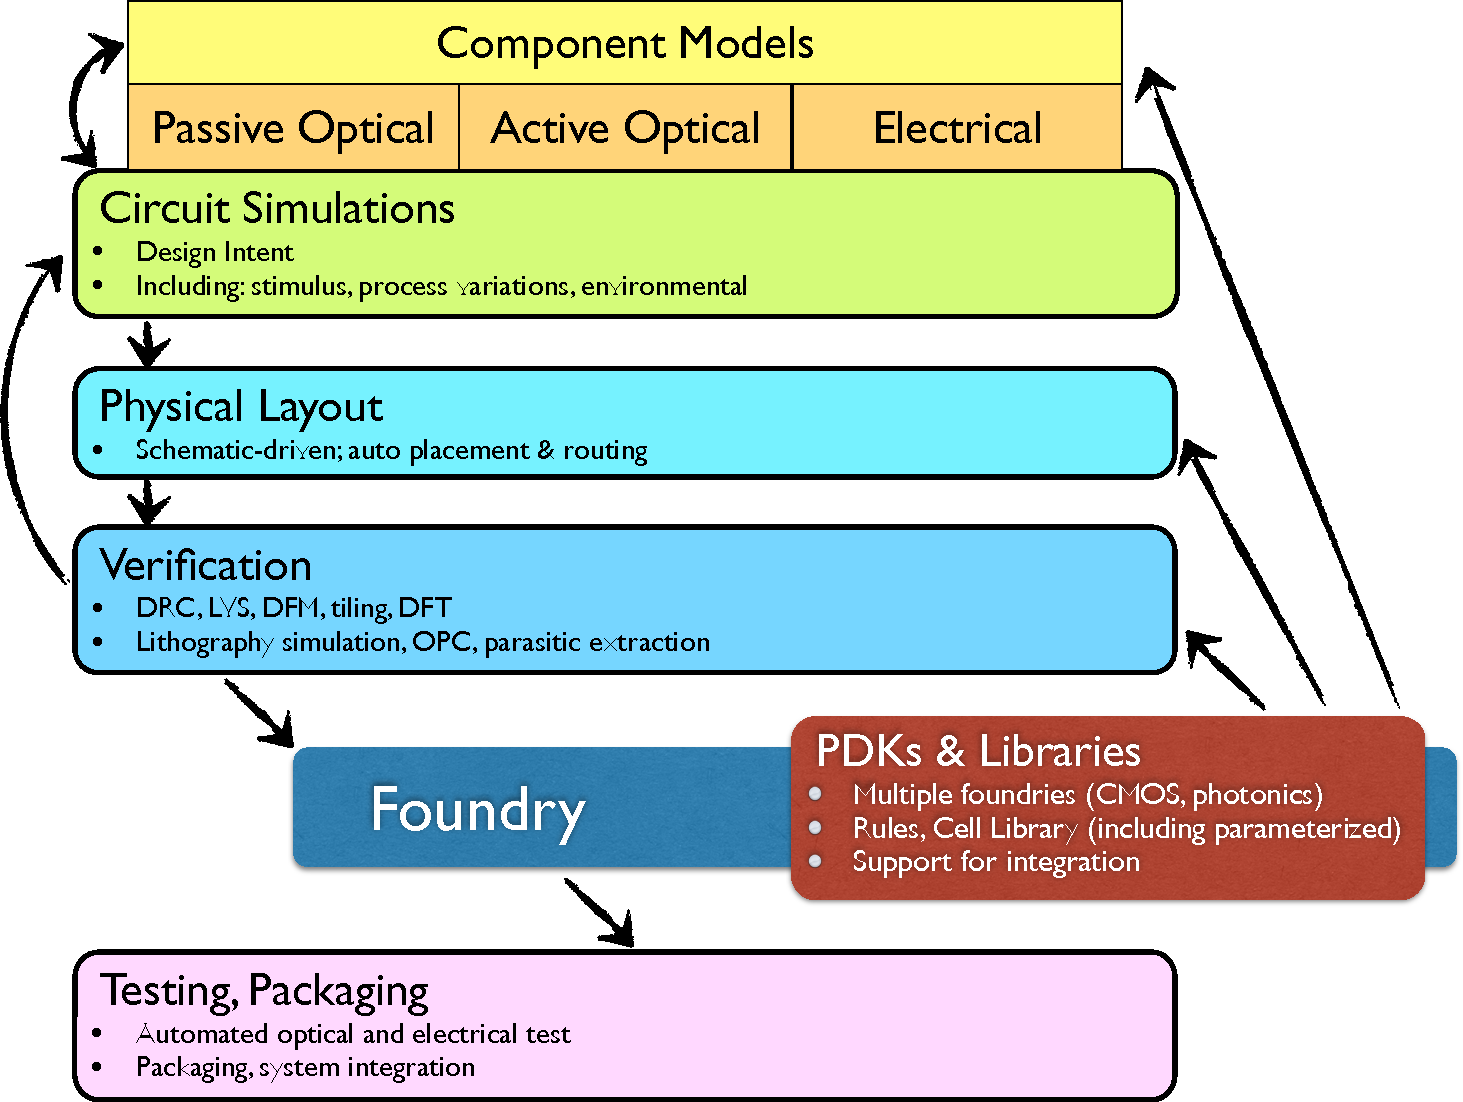
\includegraphics[width=0.7\textwidth]{../figs/SiliconPhotonicsDesign_Overview-crop.pdf}
        \caption[]{Graphical overview of a silicon photonic system design workflow, starting from the simulation of individual devices, the circuit simulations, verification, fabrication, testing, and packaging.  The flow is supported by foundry-provided design rules and component libraries. 
}
        \label{SiliconPhotonicsDesign_Overview}
\end{figure}


Full silicon photonic design flows have and are being developed by several groups, including Luxtera, IPKISS, and PhoeniX.  IPKISS software is implemented in Python, and offers a unique design flow that is available via a web browser.  The design flow presented here uses  a conventional EDA design flow, similar to the approach taken by Luxtera.  Given that one goal is electronic-photonic integration, we have chosen to use a set of Linux-based electronic design automation tools from a major vendor, Mentor Graphics, together with compatible optical circuit and component modelling software, from Lumerical Solutions.


\subsection{Generic Silicon Photonics PDK}\label{GSiP}

In this section, we describe a Generic Silicon Photonics (GSiP) PDK, which is implemented in Mentor Graphics  (Pyxis and Calibre) and Lumerical INTERCONNECT tools and is available for download at \url{http://www.siepic.ubc.ca/GSiP}.  The purpose of this kit is to demonstrate the functionality of a silicon photonics design flow implementation, with no restrictions to its distribution.  This kit can be adapted for different fabrication processes, and also provides insight into what PDK and Libraries available today offer, % \cite{opsis, siepic_www}.
namely in the NSERC CREATE Silicon Electronic Photonic Integrated Circuits (SiEPIC) program and the Optoelectronic Systems Integration in Silicon (OpSIS) foundry service. 

The components of the GSiP PDK include:
\begin{itemize}
	\item Fabrication process parameters, mask layer table
	\item Library: a small example library of components, including fibre grating couplers; waveguides, waveguide bends, and a splitter; a ring modulator; and a electrical bond pad.  
	\begin{itemize}
		\item Component symbols for schematic capture: using the Library components and/or user-provided components, circuits can be designed at the schematic level
		\item Component models: the Library components include circuit models implemented in Lumerical INTERCONNECT.
		\item Component physical layout: mask layout for components is implemented in fixed-layout cells (i.e., GDS, e.g., y-branch splitter) and parameterized (i.e., PCells, e.g., ring modulator). 
	\end{itemize}
	\item Schematic Capture: This functionality allows the designer to create a schematic of their system.  This stage of the design includes defining the connectivity between components (netlist), labelling components and ports, and choosing parameters for the PCells.
	\item Circuit simulations: The schematic is exported as a netlist, and loaded in the circuit simulation tool, Lumerical INTERCONNECT.  Component models are loaded from the Library.  The connectivity is imported from the netlist.  A simulation test-bench can be defined to perform specific simulations, such as optical transmission spectrum, time domain characterization, etc.  Functionality of the system can be simulated and verified.
	\item Schematic-Driven Layout (SDL):  The components and connectivity are imported from the schematic and (automatically) instantiated.  The connectivity is graphically represented.  The interactive (or automated) routing tool is used to complete the metal and optical routing.
	\item Waveguide routing: Electrical routing has been largely automated in the EDA tools.  In photonics designs, the tool needs additional considerations for smooth waveguide bends,  different types of waveguides,  wide low-loss waveguides for long distance routing, and waveguide crossings.

	\item Design Rule Checking (DRC): Foundry supplied rules include minimum feature size, minimum spacing, inclusion and exclusion rules.  Basic rules are included in this PDK for typical minimum feature sizes.  These rules are primarily concerned with what is permitted by the foundry to yield a manufacturable design.   %The rule checker operates in two modes: 1) Interactive -- as the layout is constructed, the tool graphically reports the errors; this allows the designer to correct the errors immediately during layout.   Interactive checking operates on a small fraction of the layout, namely the portion of the layout that is being edited and in view.  2) Sign-off verification -- the full layout is exported and checked for errors.  An error report is provided graphically and as a list.
	\item Layout Versus Schematic (LVS):  While DRC identifies errors that violate manufacturing rules, it does not identify circuit or construction errors.  LVS plays this role, by comparing the schematic and the physical layout.  It operates on the layout and identifies components and connections, creates a netlist, and compares the netlist with the original design schematic.  It identifies circuit differences, to isolate errors such as net errors (broken waveguides or metallic interconnects, disconnected optical and electrical ports, accidental crossings of interconnects), and component errors (missing components, incorrect component placed, wrong PCell parameters such as incorrect ring resonator radius).
	\item Tiling: One of the manufacturability design rules concerns the density of the patterns.  In order to meet the minimum density rules, tiles are added to the layout, typically to the silicon and metal layers.  This is necessary to ensure planarity during the chemical mechanical polish (CMP) fabrication step, and also to have an etch density that is as uniform as possible leading to reduced process variability.  This GSiP PDK does not include the tiling script as it uses a propriety language.  
	\item Sub-system design example and tutorial: a 2-channel wavelength division multiplexed (WDM) optical transmitter using ring modulators.  Example includes schematic, circuit simulations including optical spectra and eye diagrams, schematic-driven layout, design rule checking, layout versus schematic, and post-layout extraction.
	\item Electronic / Photonic co-Design: The GSiP PDK contains both an optical and electronic generic technology, which enables two separate chips to be co-designed.  
\end{itemize}





\begin{figure}[tbp]
\centering   
\subfloat[Fibre grating coupler]{\label{symbol_GC} 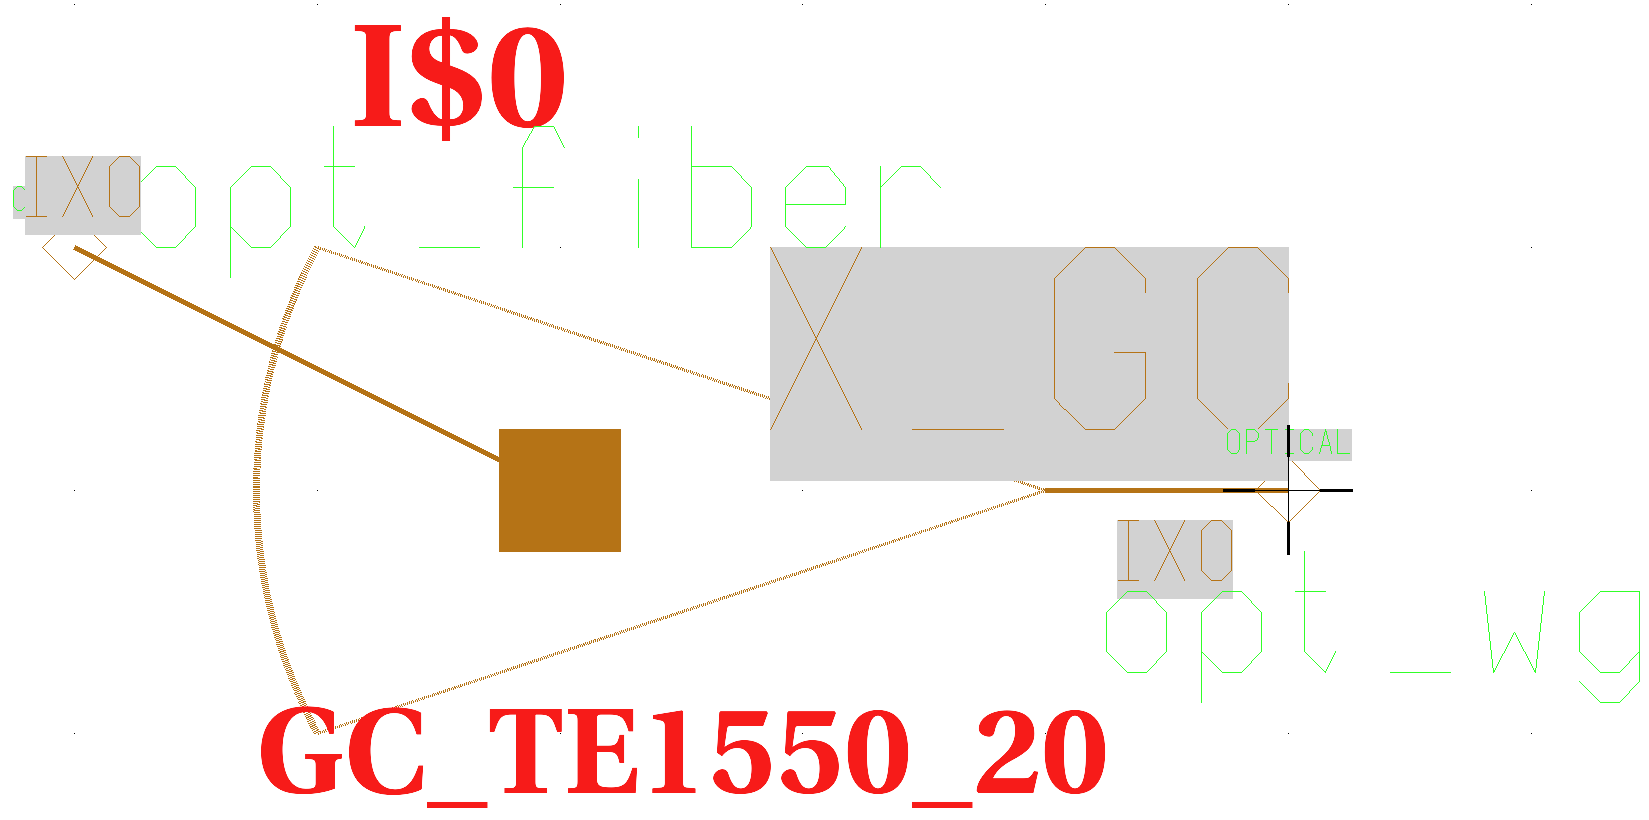
\includegraphics[width=0.3\linewidth]{../figs/symbol_GC} } 
\subfloat[Bond Pad]{\label{symbol_BondPad} 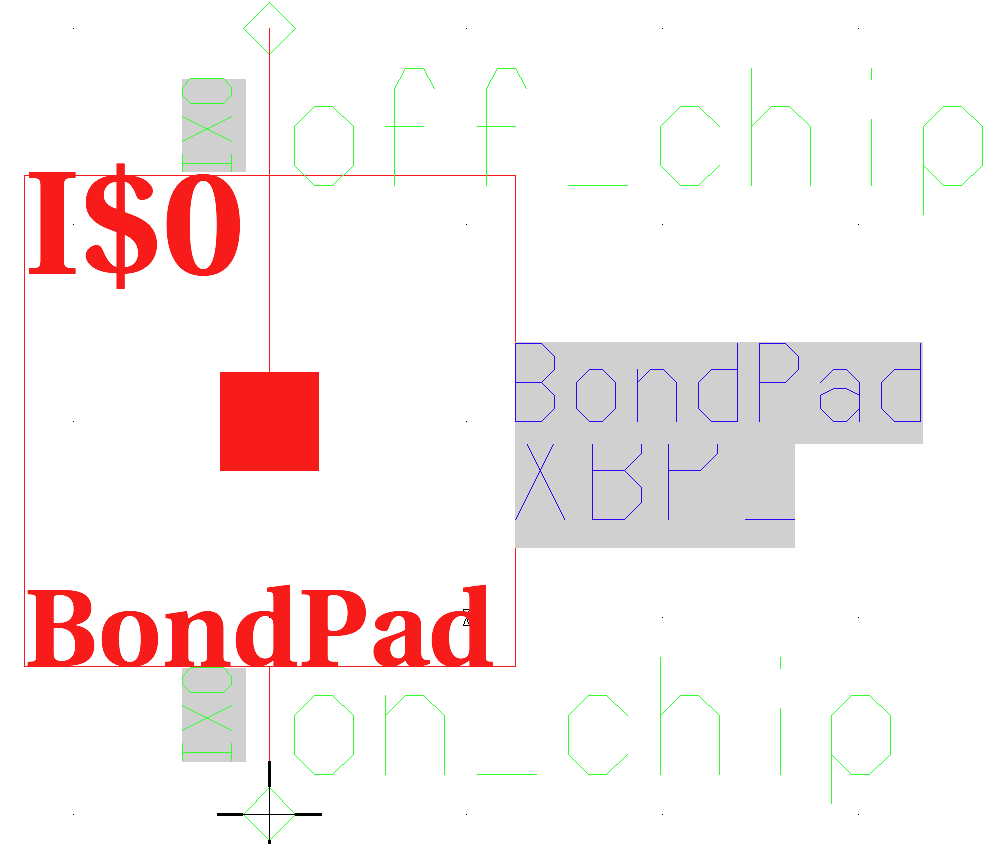
\includegraphics[width=0.22\linewidth]{../figs/symbol_BondPad} } \\
\subfloat[Y-Branch]{\label{symbol_YBranch} 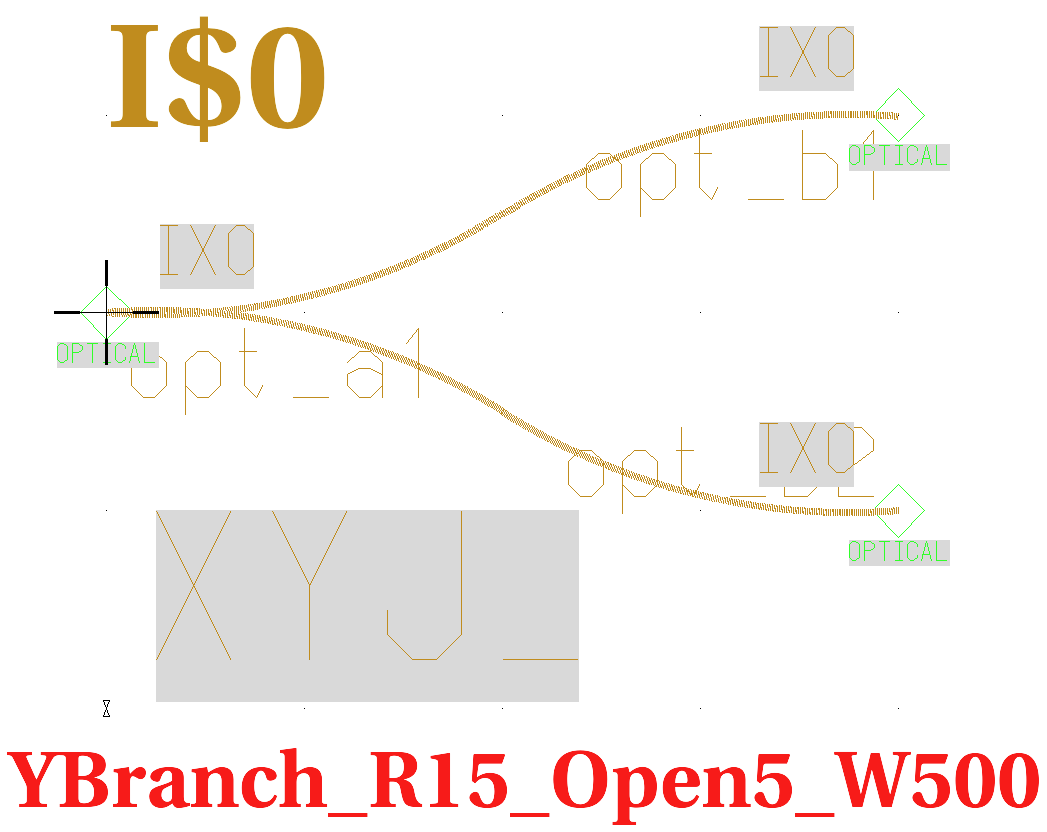
\includegraphics[width=0.3\linewidth]{../figs/symbol_YBranch} } 
\subfloat[Ring Modulator]{\label{symbol_RingMod} 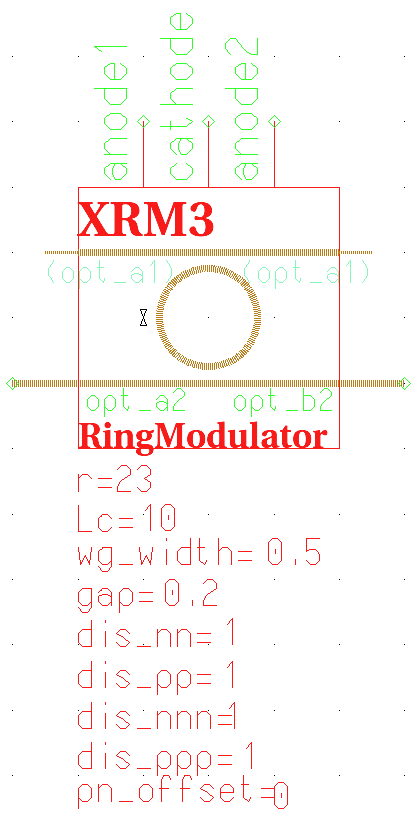
\includegraphics[width=0.2\linewidth]{../figs/symbol_RingMod} } 
\caption{Schematic symbols for library components.}
\label{Symbols}
\end{figure}






\section{Schematic Capture} 

Figure~\ref{Symbols} shows examples of schematic symbols in the Library.   As an example, the library includes a parameterized double-bus racetrack modulator (can be a point-coupled ring modulator).  The parameters for this device include: radius, directional coupler gap and length, waveguide width, parameters controlling the dimensions of the doped regions, and a pn-junction offset relative to the centre of the waveguide.

The schematic diagram for a 2 channel optical transmitter is shown in Figure~\ref{schematic_wdm2tx}.  Components are instantiated using a symbol selector or searching through the Library.  Wires are added to connect the components (both optical and electrical connections).  The interface signals to the chip (bond pads, grating couplers) are established by labelling the pin nets, and adding input/output ports.   

The schematic is further updated to insert ``pwg'' waveguide devices between components to help track the total routed waveguide lengths in the layout.  The ``pwg'' device is used in the layout for waveguide routing and post-layout extraction.  This functionality can be used to impose routing constraints or initial waveguide length estimates.

\begin{figure}[tbp]
\centering
 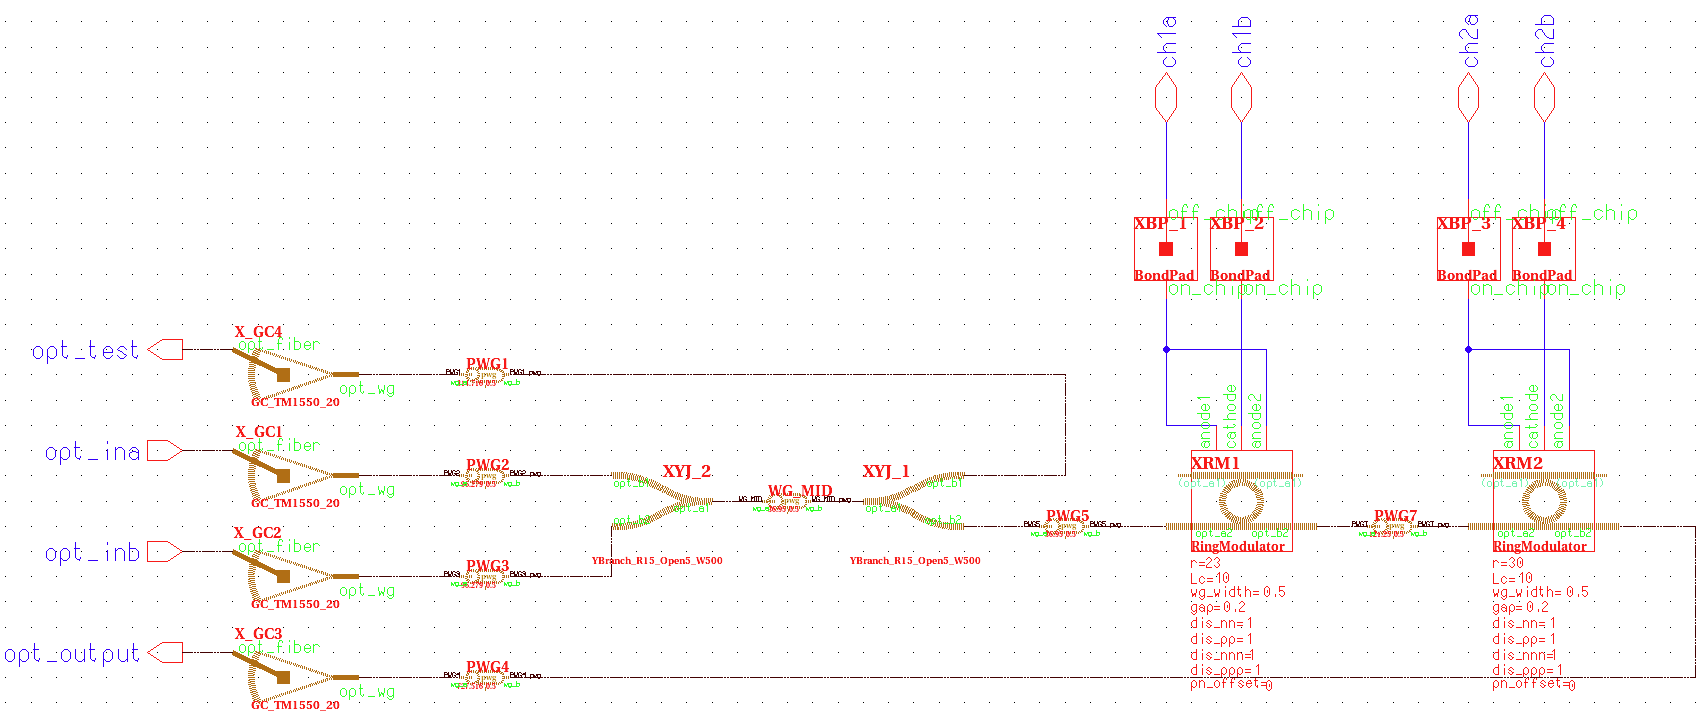
\includegraphics[width=1\linewidth]{../figs/schematic_wdm2tx}
\caption{Schematic for the example system.}
\label{schematic_wdm2tx}
\end{figure}

The schematic is checked for errors and saved.  The optical signals are annotated with a different colour to distinguish from the electrical signals.  Additionally, rule checks ensure that optical signals are  point to point and run only between optical pins.  



\subsection{Circuit Export}  

Pyxis exports a netlist of the schematic for circuit simulations.  The format for the netlist is chosen to be based on SPICE.  The schematic is represented as a sub-circuit (.subckt command), with the input/output terminals defined.  Next, each component is instanced, using a format consisting of a unique label (e.g., XYJ\_2); a series of nets this component is connected to; and the library component name (e.g., YBranch\_R15\_Open5\_W500).  The library component name is common throughout the library (symbol, simulation compact model, layout).  Parameterized cells (e.g. RingModulator) have additional parameters and values listed (e.g., r=30).



\section{Photonic Circuit Modelling}


For designing silicon photonic circuits containing numerous components, there are several approaches and tools available.    The general idea is to build simple models for components.  The simulations thus focus on the functionality and performance of the entire circuit.  
%
Many methods are available for implementing compact models for simulating devices and sub-systems that either have analytic solutions (e.g., 1 dimensional structures such as thin-film filters), or for systems that are physically too large to be effectively handled by numerical methods.  In the latter, phenomenological models, such as parameterized waveguides, can be used to simplify the simulation of larger circuits.
%
Desired simulations include frequency-domain response of the system (optical filter characterization) and time-domain simulations (transient, eye diagram, bit error rate).  The reader may be interested in journal papers that describe optical circuit modelling methods \cite{fiers2012time-domain, melati2012validation, shibata1998generalized-scattering-matrix}.  

For optical circuit modelling, the choices include: building simple circuit models in a programming language, e.g., in Matlab \cite{wartak2013computational}; using open-source solutions such as the Python-based Caphe from University of Ghent \cite{fiers2012time-domain}; implementing optical models in an EDA environment, such as the Luxtera approach using VerilogA \cite{pinguet2011cmos}; and using one of numerous commercial tools for simulating the steady-state response such as the Advanced Simulator for Photonic Integrated Circuits (ASPIC), using tools for time-domain modelling, such as Photon Design PICWave and Optiwave OptiSystem, and using tools that simulate both the time-domain and frequency-domain circuit response, including Synopsys RSoft OptiSim and ModeSYS, VPIsystems VPItransmissionMaker and VPIcomponentMaker Photonic Circuits, Lumerical INTERCONNECT, Caphe \cite{fiers2012time-domain}, and others.  

The optical circuit modelling tool used is Lumerical INTERCONNECT.  This is a photonic integrated circuit design software package that allows for the design, simulation and analysis of integrated circuits, silicon photonics, and optical interconnects containing such devices as Mach Zehnder modulators, coupled ring-resonators and arrayed waveguide gratings. INTERCONNECT includes both time and frequency domain simulators. In the time domain, the simulator calculates each element in order to generate time domain waveform samples and propagate them bidirectionally. Very close coupling between components can be simulated allowing, for example, the analysis of optical resonators. Frequency domain simulation is performed using scattering data analysis to calculate the overall circuit response. It is done by solving a sparse matrix that represents the circuit as connected scattering matrices, each one of them representing the frequency response of an individual element.  The individual elements can be built using experimental data, analytic or phenomenological models, or numerically calculated models (e.g., by FDTD or mode solver).


\subsection{Electronic-Photonic Co-Design}



For silicon photonic systems, there will often be an electronic chip.  In many cases, these can be designed separately.  
The GSiP PDK provides for data exchange between the optical and the electrical simulations.  Namely, one can design a CMOS modulator driver, and the resulting waveform can be used to drive the modulator.  Similarly, the light received by the detector is converted to a photo-current, which drives the trans-impedance amplifier.  With this approach, it is possible to design a complete CMOS-to-photonic-to-CMOS transmitter/receiver.  In this flow, both the photonic and electronic generic PDKs can be replaced with actual foundry-provided PDKs, which offers the designer flexibility in choosing which foundries are used to fabricate each of the two chips.  

This design flow is presently based on data exchange, hence does not offer co-simulation of electronics and optics, hence would not be suitable for the simulation that require lock-step self-consistent simulations, such as microwave photonic electro-optical oscillators.  For such designs, this leads to the choice of starting with a well established electronics tool (e.g., Cadence) and adding the optical functionality within the constraints of the electronic modelling approach (e.g., VHDL, Spice, VerilogA), or to start with a tool focused on optical simulations, and add on electronic modelling capabilities.   The electronic-tool approach was implemented in Cadence by Luxtera using VerilogA \cite{pinguet2011cmos}.  The photonic-tool approach is available in tools such as Synopsys RSoft OptiSim and Optiwave OptiSPICE \cite{gunupudi2010self-consistent}.  Finally, in the future there may be a third solution, namely where advanced EDA tools are coupled with advanced photonic simulation engines, for electronic-photonic co-simulation.  %The coupling can be via data exchange to simulate systems such as transceivers which use CMOS drivers, modulators, optical transmission, detectors and CMOS receivers.  %Some systems may require stronger coupling such as opto-electronic oscillators.



\subsection{Component Models for Circuit Design}

Numerical methods such as finite difference time domain (FDTD) and eigen-mode solvers coupled with solutions to optoelectronic equations are workhorses in silicon photonic component-level design.  These methods unfortunately do not scale well as the number of components in the photonic circuit increases (e.g., doubling the volume in an FDTD simulation typically increases the simulation time fourfold).  Thus, modelling approaches that are computationally efficient yet accurately represent complex nanophotonic devices need to be employed in circuit simulations.  In addition, the physical layout can affect the circuit response and needs to be considered.  These issues have been addressed by the CMOS electronics industry, and are beginning to be incorporated into silicon photonic design.  

Circuit modelling tools utilize physical-level opto-electronic simulations, and/or experimental data, to build compact models for the optical elements.  This integrated approach allows designers to study, for example, the influence of optical feedback from components such as grating couplers on the optical response of the optical circuit, taking into account the physical layout.  Such a unified methodology is essential for understanding the performance and designing for future complex silicon photonic systems.

One of the key challenges in the process is the translation from the largely geometric parameters that can be easily extracted from EDA tools and the optoelectronic parameters that are necessary for the simulation of a photonic circuit. For example, after design and layout, properties such as waveguide width, bend radius, gap distance in waveguide couplers, electrical contact positions and so on can be extracted easily from EDA tools. However, photonic circuit simulation requires optoelectronic parameters such as effective/group index, dispersion, S-parameters, and information about dependence of the effective index on applied voltage or temperature. These quantities cannot be easily determined from the geometric parameters of the layout, but require a combination of physics based solvers such as eigenmode solvers, FDTD and electrical device solvers.

%This chapter describes the process of optoelectronic parameter extraction starting from the geometric parameters in components such as waveguides, couplers, y-junctions, grating couplers, edge couplers, waveguide couplers, ring modulators, ring filters and photo-detectors. For fixed cell designs, the components can be simulated once using the appropriate physical solvers and the optoelectronic parameters can be extracted for later use. For parameterized cell designs, it is necessary to perform parameters sweeps over a range of possible geometries to create lookup tables or validated phenomenological models. We then show examples of how these extracted optoelectronic parameters can be used in photonic circuit simulations.


The designer specifies the high-level circuit parameters, known as \emph {Design-Intent Based Parameters}.  In optical circuits, this includes parameters such as the target operating wavelength, the modulation bandwidth, etc.  The design methodology enables a high-level design approach by providing appropriate compact models as well as physical implementations (layouts) of components based on these design-intent parameters.  The available components can either be discrete cells, or parameterized.  An example of such a component is the focusing fibre grating coupler, which was parameterized for wavelength, polarization, fibre angle, and all process parameters \cite{wang2013universal}.

There are several ways to represent a component in a circuit simulation.  Desirable properties for a compact model include: 1) Accuracy -- while a compact model provides enormous computation complexity savings, the circuit model needs to be sufficiently accurate; 2) Wavelength/polarization dependance -- this is necessary in order to be able to model a circuit over the wavelength range of interest.  In many cases, the wavelength dependance cannot be ignored, such as for a waveguide in a ring resonator, since it is the group index that determines the free-spectral range; 3) Parameterized versus the geometry -- a model that covers a range of physical parameters is necessary to study the circuit dependance on physical parameters, such as waveguide thickness, width, etc, including fabrication variation and non-uniformity.  This can be implemented by a collection of single-element compact models accessed via a look-up table, or a multi-dimensional parameterized model.

	Next, we describe two common methods for constructing compact models.
	
\subsection{Compact Models -- Empirical and S-Parameters}
	
Empirical models are the standard approach used in electronics design.  For example, a SPICE model for a transistor can have over 100 parameters in a suitable function that is used to fit experimental (or simulated) data. It is common in the electronics industry to create compact models extracted from experimental data.  Numerous tools can build an equivalent electrical circuit model for a set of measurements, e.g., a frequency response (e.g., Agilent Advanced Design System - ADS).  Other tools can can curve-fit the frequency response to empirical models such as polynomial or rational functions \cite{gustavsen1999rational, zeng2006modified}.  The advantage of such compact models is that they are just that -- compact -- particularly when compared to the original S-parameter measured data.  By choosing an appropriate function, the curve-fitting effectively smooths over the measurement noise, thus leading to well behaved system simulations.  These compact models are  highly suitable for large-scale system simulations.  The main challenge is identifying appropriate model equations and keeping track of the range of validity (e.g., valid frequency range).    In general, it is beneficial to have an understanding of the expected variation and to use as simple model as possible.  For example, a (linear) resistor is typically modelled by a single parameter, $R$.  If one fit experimental data with an N-order polynomial, then some measurement error would be captured by the fit possibly resulting in an incorrect model.  

Scattering parameters (S-parameters) can be used to describe the behaviour of a linear network.  Traditionally this concept is used to describe the response of electrical devices as a function of frequency.  S-parameters are particularly useful for experimental characterization of electrical devices, using a vector network analyzer (VNA).   They can also be used to describe optical devices, with experiments conducted using an optical vector network analyzer (ONA).  In both cases, measurements are performed over a range of frequencies -- typically GHz frequencies in the electrical RF domain, and THz in the optical domain.  The S-parameters are generally complex, meaning they include an amplitude response, and a phase response. 

S-parameters can  be used for system levels simulations, where multiple components can be cascaded and the overall response of the system can be very conveniently determined. S-parameters are excellent for experimental data, however the measurement data includes noise and other sources of error, which are then included in subsequent system analysis, and the parameters are measured at many frequency points (e.g., 10,000).  The use of these parameters in system modelling thus has two main challenges: the incorporation of measurement error, and computational complexity.  The computation inefficiency is particularly trouble-some for very large system modelling (e.g., thousands of optical components), and when executing time-domain simulations which require the frequency domain S-parameters to be converted into an impulse response filter (e.g., finite or infinite impulse response filters).

\subsection{S-Parameters from FDTD Simulations}

Similar to experimental results, FDTD simulations are not 100\% accurate.  There is always a residual numerical error due to the finite mesh size, spurious reflections from the simulation boundaries, etc.  Just as with experimental data, S-parameters can be extracted from FDTD simulations.  Constructing compact models from numerical simulations has the same benefits as with experimentally-derived compact models -- as an effective data reduction technique which leads to more stable and fast system-level simulations.

 To simulate the S-parameters using FDTD, first the geometry is constructed, as shown in Figure~\ref{DC_image1}. This example considers the directional coupler used in a ring modulator, with rib waveguides. The top waveguide can eventually be used to form a ring resonator, and the bottom waveguide is the coupler.

Since this is a four port device, in general four simulations would need to be conducted: input on port 1, with measurements on ports 1, 2, 3, and 4. This is followed by a second simulation with input on port 2, and so on.  However, we can often make use of symmetry to simply the measurements or simulations.  In this case, the device is symmetric about the vertical axis, hence the results for light input on port 3 would be the same as when input on port 1.

The first simulation is shown in Figure~\ref{DC_image1}.  Light is incident on port 1 using a mode source (pointing down).  Four field monitors are positioned at the four waveguides.  In addition, mode expansion monitors are used to isolate the component of the field travelling in a particular direction, and also to ensure the measurement is taking only into account the light in the fundamental mode of the waveguide. For example, to find the S11 parameters, the field monitor is above the source and measures the reflected light (travelling up in the figure).  The data in each of the monitors is then normalized to the power in the input waveguide, which results in the complex S-parameters. These can be written as magnitude and phase.  This first simulation gives the four S-parameters, S11, S21, S31, and S41.  The magnitude response is shown in Figure~\ref{S1121m}.  For a four-port device, there will be sixteen parameters.  In this example, a second simulation on port 2 is required, and symmetry can be used to fill in the remaining parameters.

There are two important considerations when working with S-parameters for optical waveguides: firstly, the waveguide modes are not necessarily power orthogonal -- meaning that the total power in the waveguide is not simply the sum of the power in each individual mode present; and, secondly, the vectorial nature of the EM modal fields introduces additional complexity compared to a scalar quantity like voltage.
\begin{enumerate}
\item Waveguide power orthogonality:

Fortunately, in non-absorbing waveguides, the waveguide modes are power orthogonal which greatly simplifies the analysis. While there is always some absorption in real waveguides, in most practical circuits it is sufficiently low that we can make the approximation that the waveguide modes are power orthogonal. Care should be exercised when this approximation is invalid.  For example, the waveguides used in many Ge photodiodes are clearly such a case.

\item Vectorial nature of waveguide modes:

In general, a standard sign and phase convention for the E and H fields of forward and backward propagating modes should be used for all ports of a component. Typically, in a non-absorbing waveguide, the transverse E and H fields are chosen to be real-valued. The backward propagating mode has the same field profile but the tangential H field and normal E field components are reversed in sign. The S-parameters are the complex coefficients of the forward and backward propagating modes, once all modes have been normalized to carry the same power. This means that the S-parameters can have additional negative signs that may not be expected. For example, the S21 in a 180 degree U-bend will have an additional negative sign for TE-like modes but not for TM-like modes, see Figure~\ref{EM}.  This is simply due to the fact that the physical fields in the waveguide are the S-parameter coefficients multiplied by the (fully vectorial) modal fields of the waveguide and a 180 degree rotation will reverse the direction of some field components. Furthermore, we must be careful when using symmetry considerations to reduce the number of simulations or measurements that need to be made since the symmetry of the modal fields must be considered.
\end{enumerate}

%	
%	\begin{figure}[tbp]
%		\centering
%	   \begin{overpic}[width=0.3\linewidth]{../figs/DC_diagram}
%	      \put(20,55){\huge 1}
%	      \put(7,15){\huge 2}
%	      \put(80,55){\huge 3}
%	      \put(90,15){\huge 4}
%	   \end{overpic}  \\
%		\caption{Directional coupler device and simulation configuration.}
%		\label{DC_image1}
%	\end{figure}

%\begin{figure}[htbp]
%\begin{center}   
%\subfloat[Directional coupler device and simulation configuration.]{\label{DC_image1} \begin{overpic}[width=0.3\linewidth]{../figs/DC_diagram}
%      \put(20,55){\huge 1}
%      \put(7,15){\huge 2}
%      \put(80,55){\huge 3}
%      \put(90,15){\huge 4}
%   \end{overpic}  }  \hspace{2 cm}
%\subfloat[Characterization of the directional coupler model.]{\label{DC_image}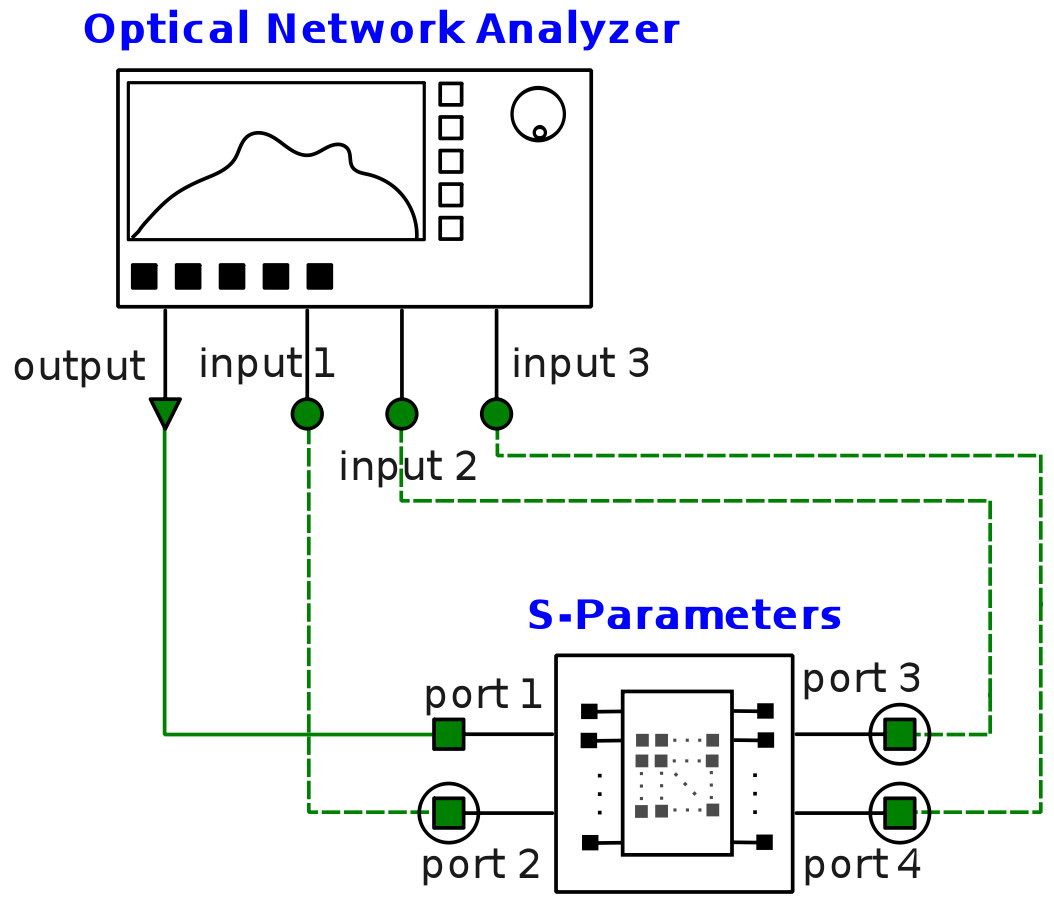
\includegraphics[width=0.25\linewidth]{../figs/INT_ONA_DC} } \hspace{2cm} 
%\caption{Circuit modelling schematic diagrams, in Lumerical INTERCONNECT.  The S-parameters for the directional coupler are used to create the model used by the simulator.  The Optical Network Analyzer is used measurement the optical transmission spectra.}
%\label{INT_DC}
%\end{center}
%\end{figure}


%
%\begin{figure}[htbp]
%\begin{center}   
%\subfloat[FDTD simulation configuration.]{\label{DC_image1} \begin{overpic}[width=0.35\linewidth]{../figs/DC_diagram}
%      \put(20,55){\huge 1}
%      \put(7,15){\huge 2}
%      \put(80,55){\huge 3}
%      \put(90,15){\huge 4}
%   \end{overpic}  }  % \hspace{2 cm}
% \hspace{1cm} 
%%\subfloat[S31, S41]{\label{S3141m} 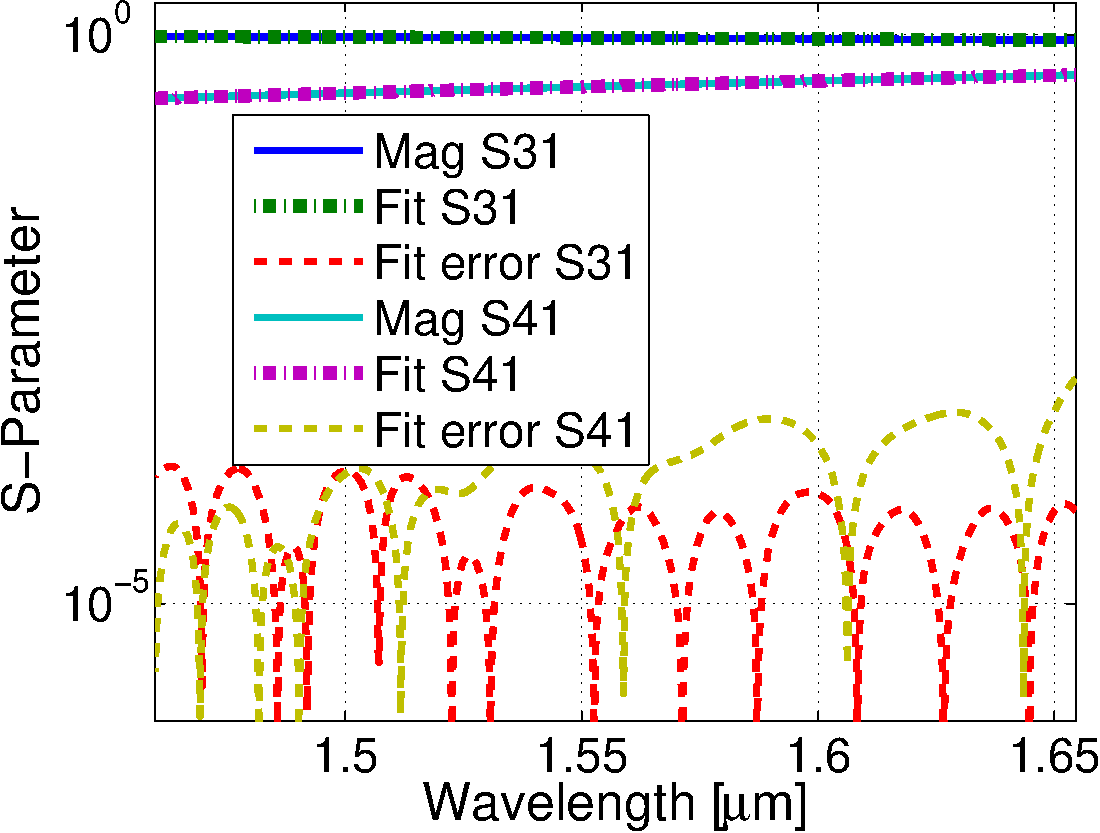
\includegraphics[width=0.48\linewidth]{../figs/DC_ringmod_type1_R=10,gap=180,Lc=0,wg=500,lambda=1550,mesh=2,angle=30,mat_abs_S31_S41} }
%\subfloat[Simulated S-parameters (magnitude)]{\label{S1121m} 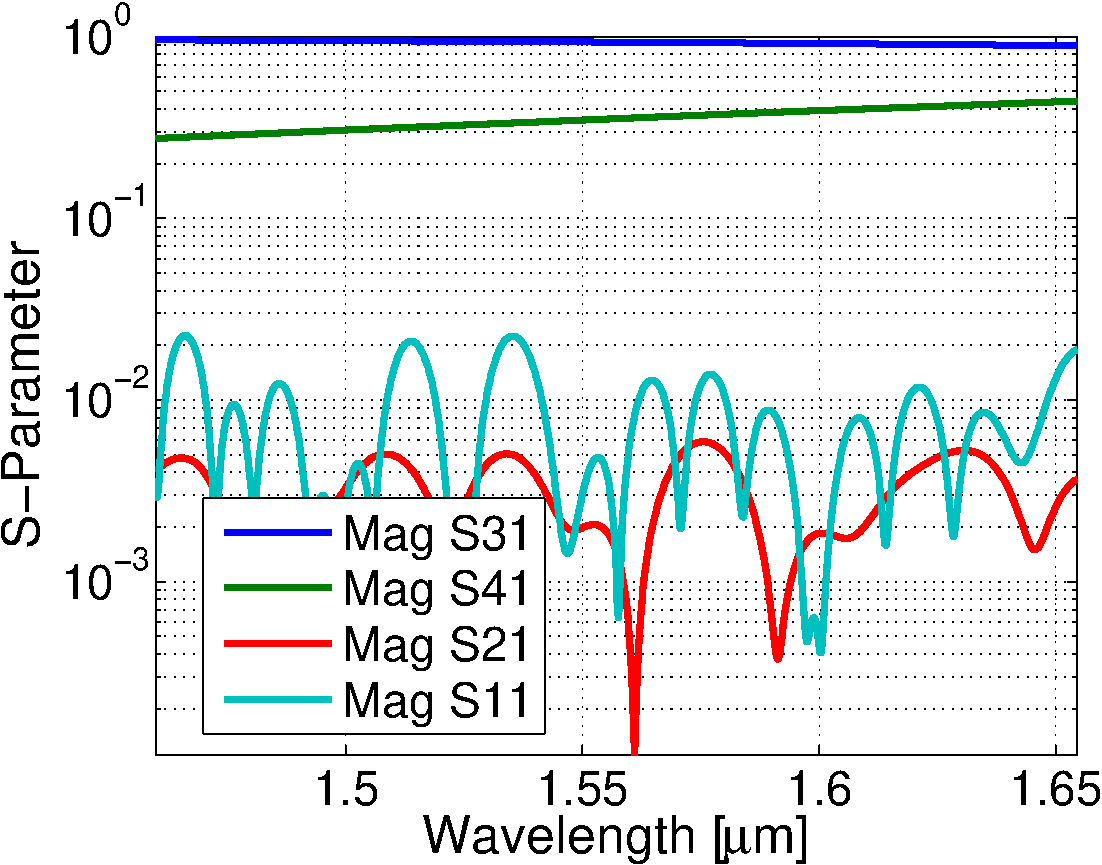
\includegraphics[width=0.48\linewidth]{../figs/DC_ringmod_type1_R=10,gap=180,Lc=0,wg=500,lambda=1550,mesh=2,angle=30,mat_abs_S21_S11_spie} } 
%\caption{Directional coupler component.  }
%\label{SParam_DC_mag}
%\end{center}
%\end{figure}

\begin{figure}[htbp]
\begin{center}   
\subfloat[FDTD simulation configuration.]{\label{DC_image1} \begin{overpic}[width=0.4\linewidth]{../figs/DC_diagram}
      \put(20,55){\huge 1}
      \put(7,15){\huge 2}
      \put(80,55){\huge 3}
      \put(90,15){\huge 4}
   \end{overpic}  }  % \hspace{2 cm}
 \hspace{1cm} 
%\subfloat[S31, S41]{\label{S3141m} 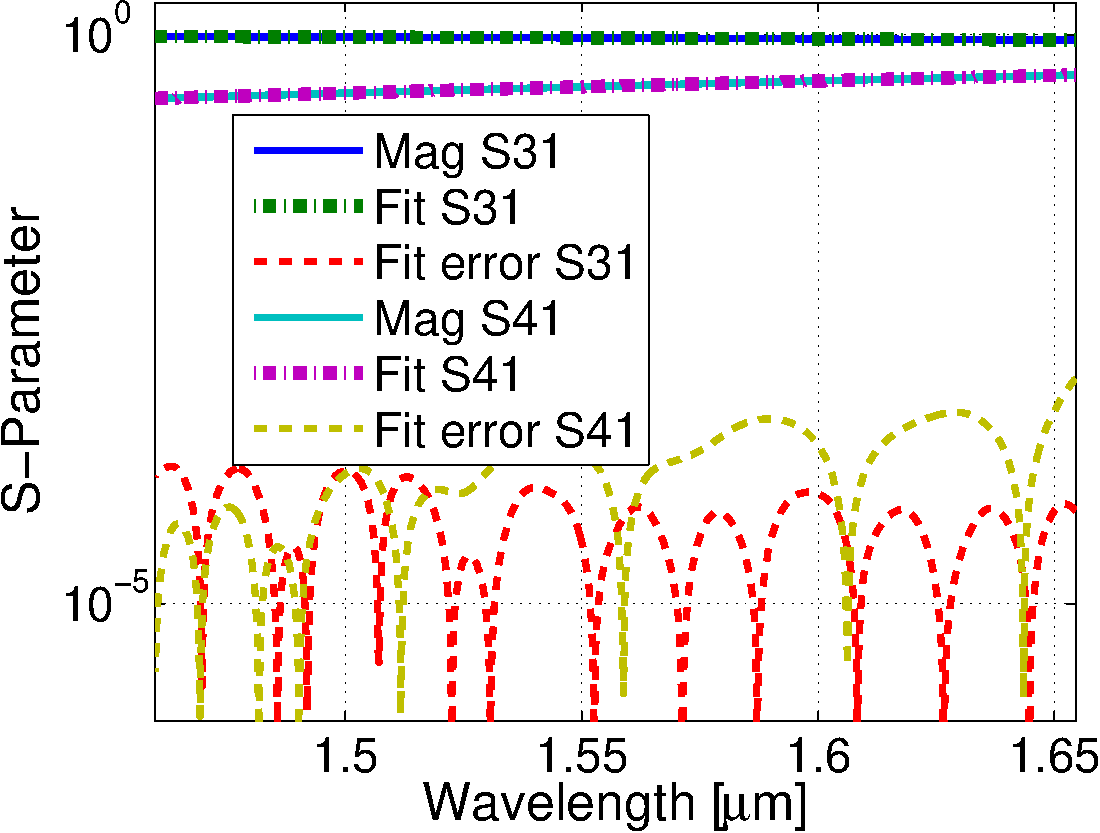
\includegraphics[width=0.48\linewidth]{../figs/DC_ringmod_type1_R=10,gap=180,Lc=0,wg=500,lambda=1550,mesh=2,angle=30,mat_abs_S31_S41} }
 \hspace{1cm}
\subfloat[EM-field considerations for defining S-parameters.]{\label{EM} 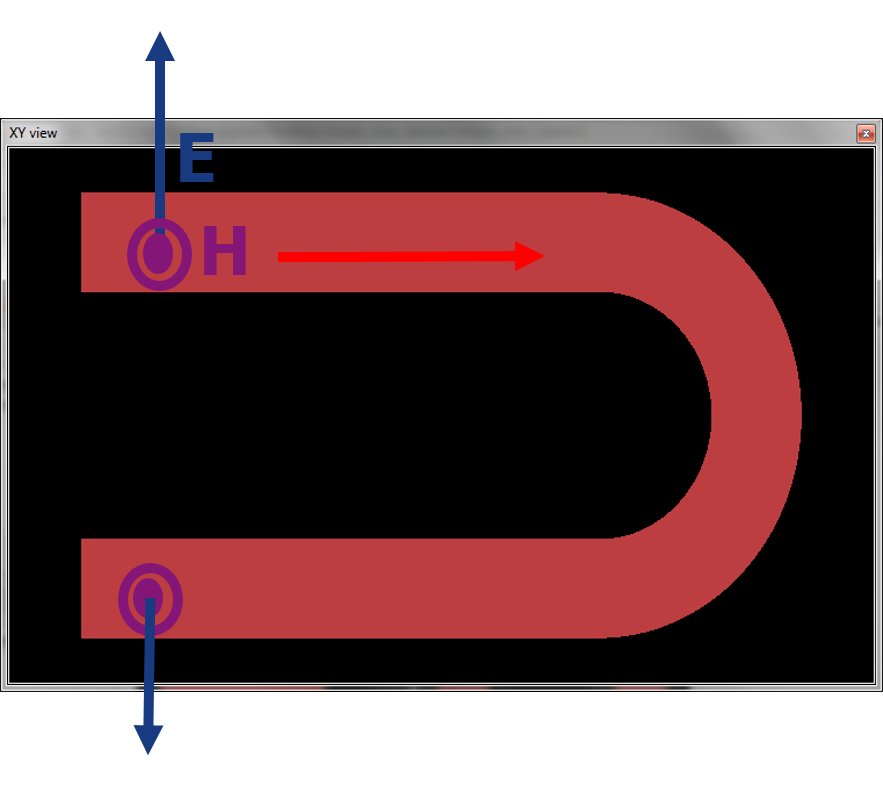
\includegraphics[width=0.4\linewidth]{../figs/Picture1.png} } 
\caption{Simulation configuration diagrams.  }
\label{figb}
\end{center}
\end{figure}

%Efficient circuit simulations can be by achieved by using S-parameters directly.  This is particularly simple for the optical transmission response of an optical circuit, built using components with known S-parameters.  For time domain simulations, the circuit modelling tool internally needs to convert the S-parameters into a time-domain representation.  In this section, we use the results of the FDTD simulations in a circuit simulation, using Lumerical INTERCONNECT.  

\subsubsection{Passivity Assessment}

When importing S-parameters for system simulations, it is necessary to ensure that the parameters are passive, namely that the model does not generate energy.  This would clearly be problematic for structures such as ring resonators and result in non-physical results where gain may be  observed in the simulations.  
%In order to use S-parameters of passive optical components in circuit simulations, we first need to make sure that the parameters are valid, namely that they meet the passivity requirements.  
A passive model needs to be stable (impulse response decays in time), and passive (no amplification).  Ideally it should also be causal (impulse response is 0 for t$<$0). 
One test that can be applied to the S-parameters is the norm-2 test, which verifies if the system is passive, namely:
\begin{equation}
	||S(j\omega)||_2 \le 1
\end{equation}

For the S-parameters shown in Figures~\ref{S1121m}, the passivity test is performed for the 4x4 complex S-parameter matrix for each wavelength.  The result is plotted in Figure~\ref{DCSparam_passivity3}.  As can be seen, the result is greater than 1 for some wavelengths.  Thus, the model is not passive, hence, these parameters should be used with caution.  S-parameters are often not passive as a result of error, either measurement, or in this case, numerical, error.  In these cases, small adjustments can be made to force passivity, as described next.


\subsubsection{Passivity Enforcement}

One approach to force passivity is to employ the rational modelling techniques provided open-source by B.~Gustavsen, to condition the S-parameters.  The approach is as follows:

\begin{enumerate}
	\item Assess the passivity of the S-Parameters \cite{gustavsen2008fast}.  If it is not passive, then
	\item Curve-fit the S-parameters to a rational function with a series of poles using the Vector Fitting technique \cite{gustavsen1999rational,gustavsen2006improving, deschrijver2008macromodeling}:
		\begin{equation}
			\mathbf{S}(s) = \sum_{m=1}^N \frac{\mathbf{R}_m}{s-a_m}
			\label{EQ-VF}
		\end{equation}
		where $\mathbf{S}(s)$ are the S-parameters; $s=j 2 \pi f$ is the complex frequency, with $f$ being the optical frequency; $a_m$ are the poles; $\mathbf{R}_m$ are the residues matrices.
	\item Obtain a passive version of the pole-residue function, by perturbing the model until it becomes passive \cite{gustavsen2010fast}.
	\item The pole-residue compact model can be used directly in circuit simulations, can be converted into a lumped equivalent circuit model \cite{gustavsen2002computer}, or the S-parameters can be generated and exported.  The choice depends on the tool preference.  
	
\end{enumerate} 

%\begin{figure}[tbp]
%	\centering
%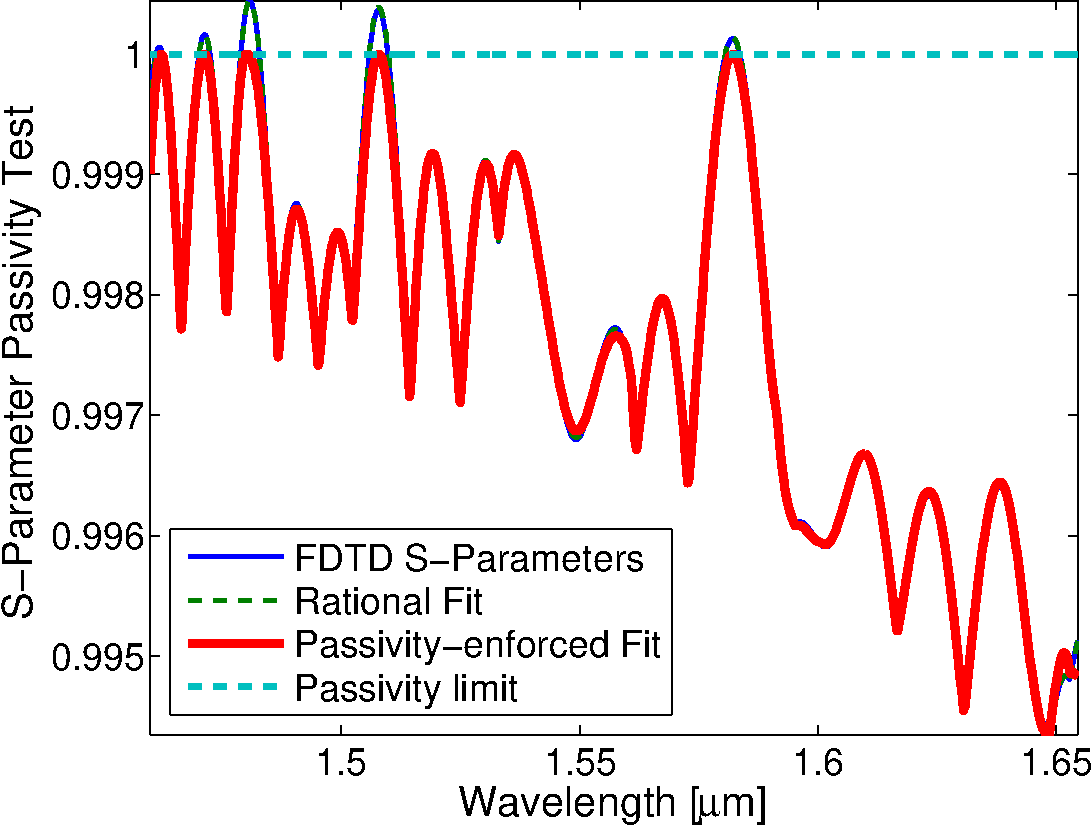
\includegraphics[page=1,width=0.5\linewidth]{../figs/DC_ringmod_type1_R=10,gap=180,Lc=0,wg=500,lambda=1550,mesh=2,angle=30_passivitytest3} 
%	\caption{Passivity test on the S-parameters before and after Vector Fitting and Passivity Enforcement.  The S-parameters have been made passive for all frequencies.  }
%	\label{DCSparam_passivity3}
%\end{figure}

\begin{figure}[tbp]
\begin{center}
\subfloat[Simulated S-parameters (magnitude).]{\label{S1121m} 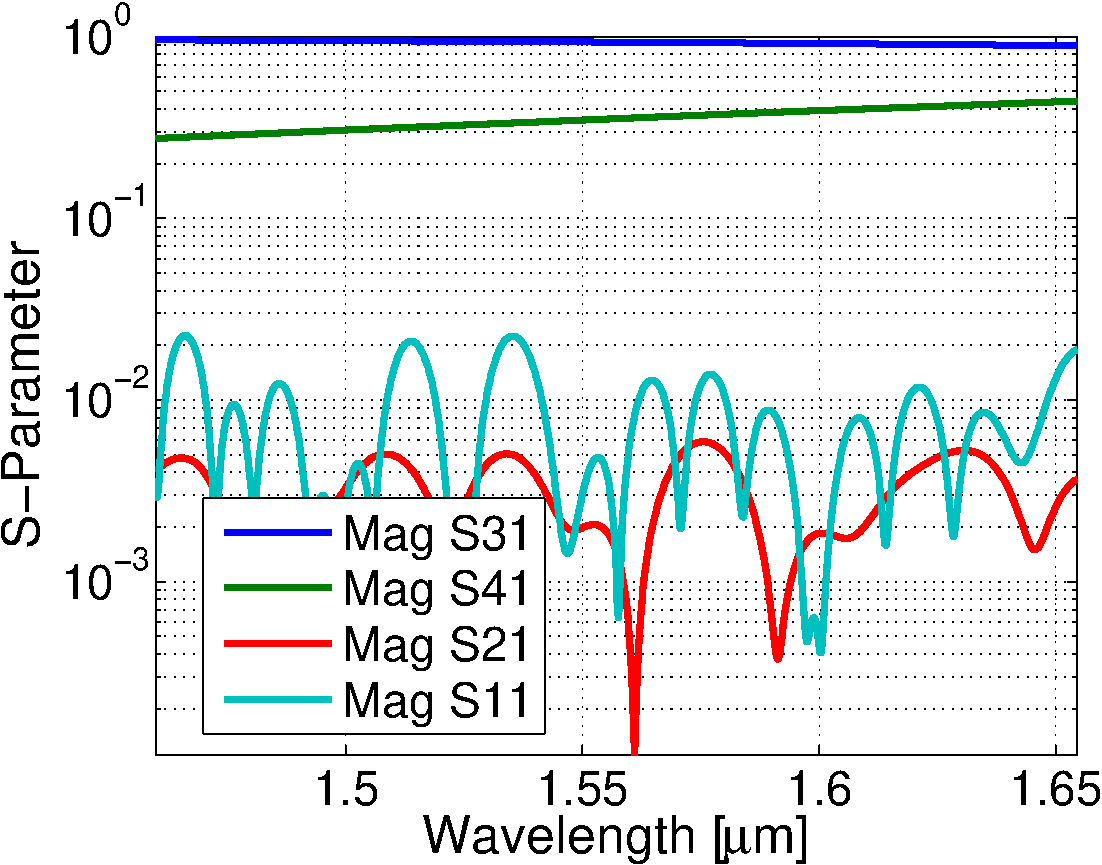
\includegraphics[width=0.48\linewidth]{../figs/DC_ringmod_type1_R=10,gap=180,Lc=0,wg=500,lambda=1550,mesh=2,angle=30,mat_abs_S21_S11_spie} }  ~ 
\subfloat[Passivity test on the S-parameters before and after Vector Fitting and Passivity Enforcement.  ]{\label{DCSparam_passivity3} 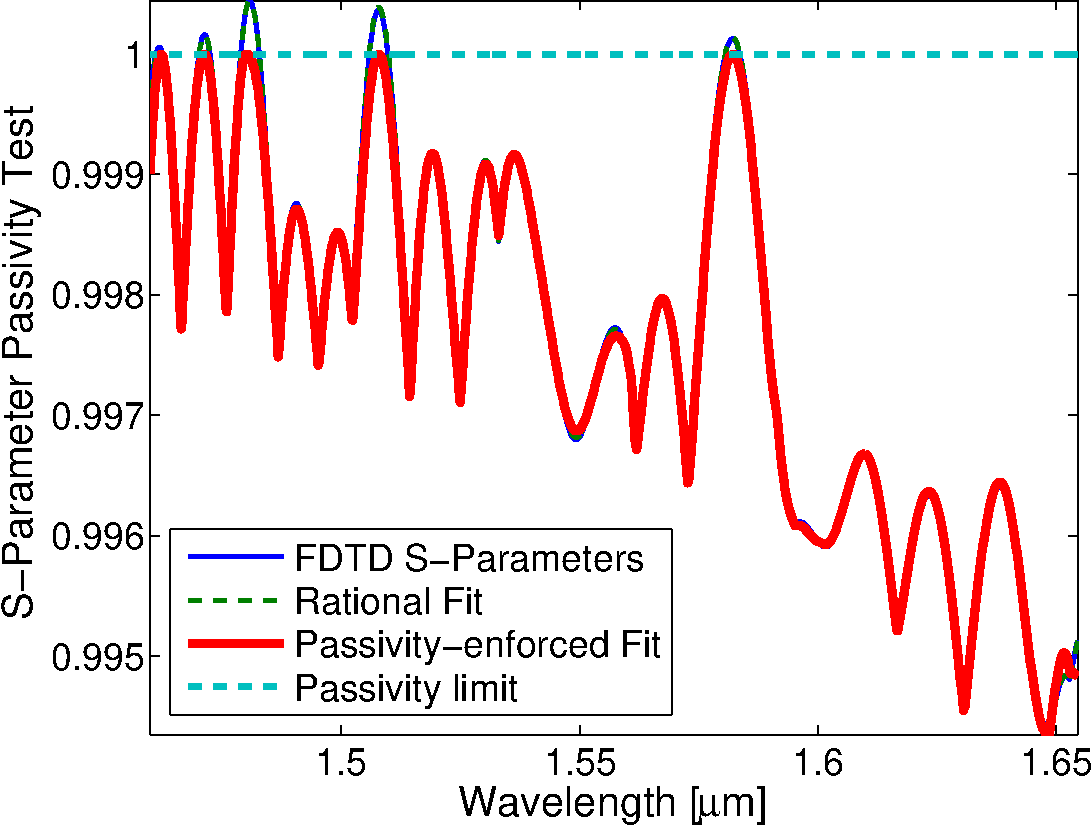
\includegraphics[page=1,width=0.48\linewidth]{../figs/DC_ringmod_type1_R=10,gap=180,Lc=0,wg=500,lambda=1550,mesh=2,angle=30_passivitytest3} 
 } 
	\caption{Directional coupler S-parameters and passivity test.  The S-parameters have been made passive for all frequencies.  }
	\label{figa}
	\end{center}
\end{figure}

\begin{figure}[tbp]
\begin{center}   
%\subfloat[Characterization of the directional coupler model.]{\label{INT_ONA_DC} 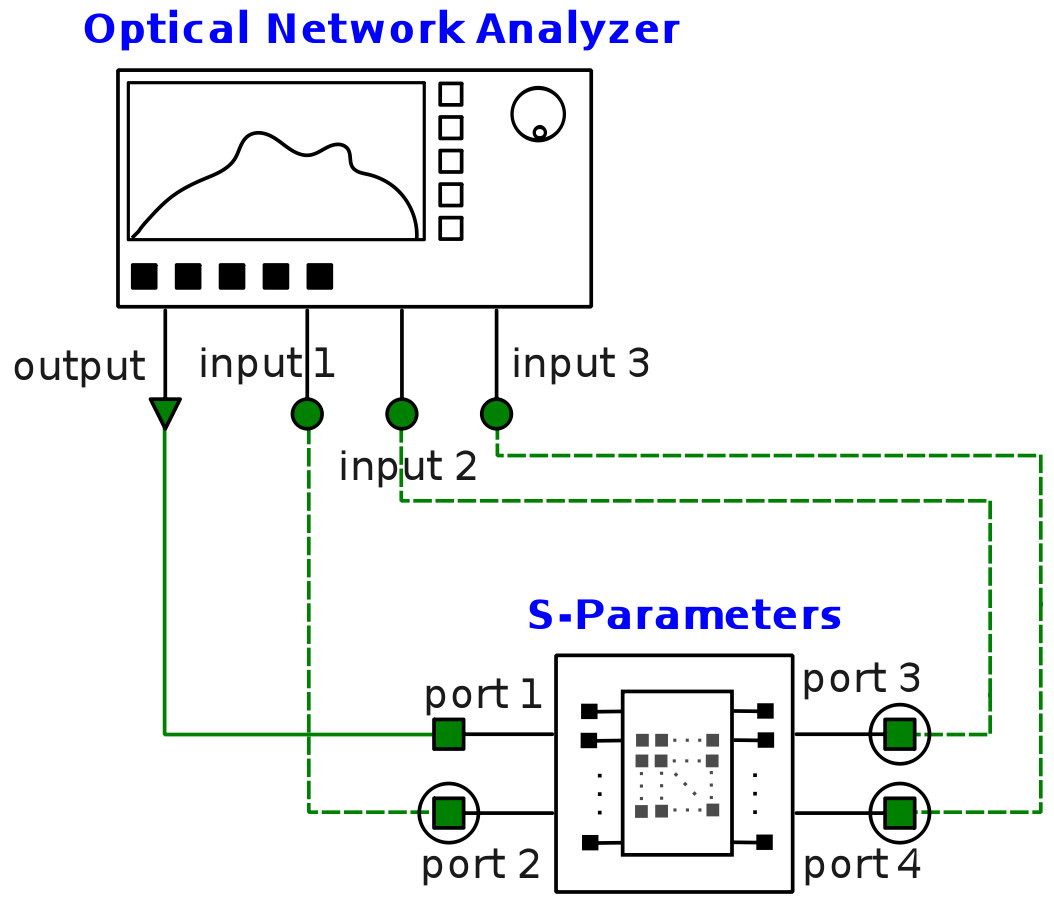
\includegraphics[width=0.25\linewidth]{../figs/INT_ONA_DC} } \hspace{2cm} 
\subfloat[Schematic diagram, tested with an Optical Network Analyzer.]{\label{INT_ONA_DCring} 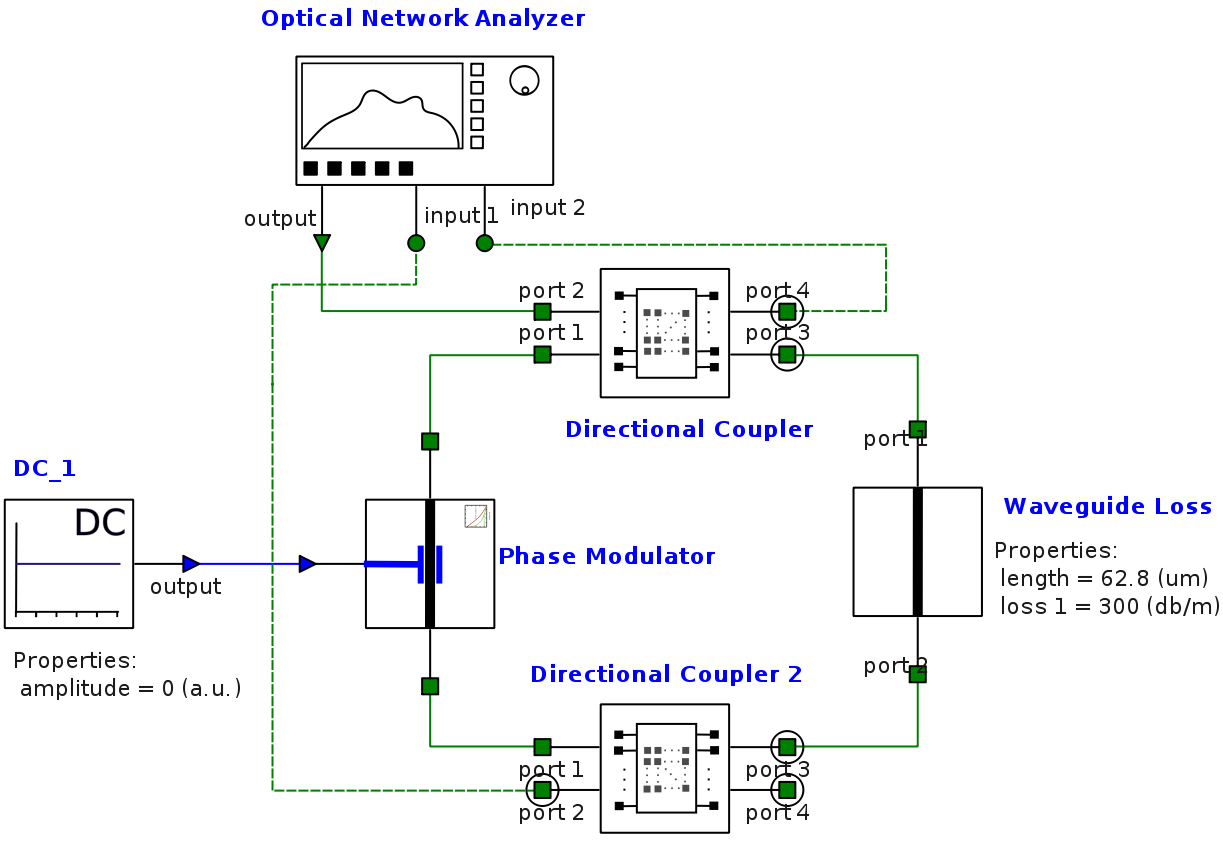
\includegraphics[width=0.5\linewidth]{../figs/INT_ONA_DCring2} } ~ ~ ~
\subfloat[Optical spectrum of the circuit.] {\label{INT_ONA_DCring}
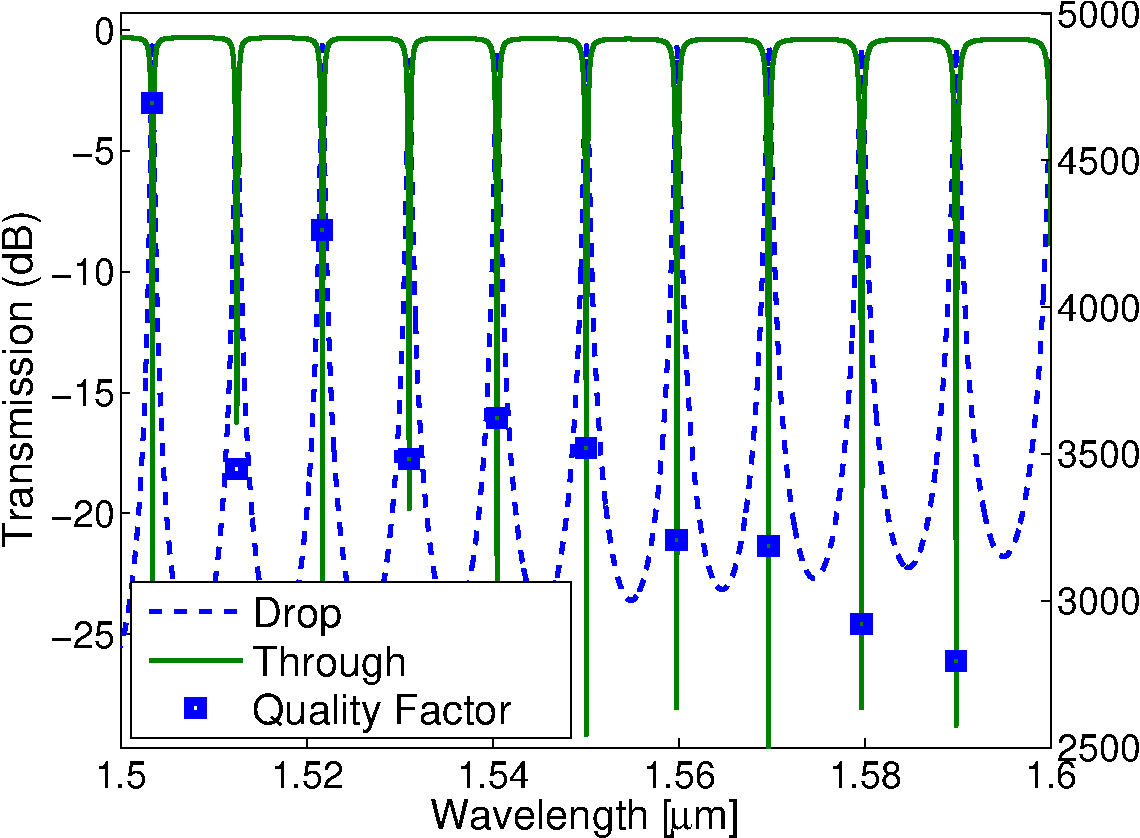
\includegraphics[width=0.3\linewidth]{../figs/a_1} }
\caption{Circuit modelling of a ring modulator constructed with two directional couplers, a phase modulator, and an additional waveguide loss.  The S-parameters for the directional coupler are used to create the model used by the simulator, Lumerical INTERCONNECT.  %The Optical Network Analyzer is used measurement the optical transmission spectra.
}
\label{INT_DC}
\end{center}
\end{figure}

Another method of passivity enforcement is to use singular value decomposition to ensure that the 2-norm of the S-parameter is always less than or equal to 1. This method is very simple and appropriate for many components where the numerical or experimental errors are small. However, it will lead to discontinuities in the derivatives of S with frequency which can be problematic for some components, particularly those with a high level of feedback. A slightly modified approach is to scale the 2-norm over all frequencies by a single value (the maximum passivity violation) which avoids any discontinuities in the derivatives.

As shown in Figure~\ref{INT_DC}, the compact models can be used to build sub-circuits in Lumerical INTERCONNECT.  We use the compact model for the directional coupler found above (passivity-enforced S-parameters) to build a ring resonator.  This is accomplished by loading the S-parameters into an Optical N Port S-Parameter import object, adding the waveguide loss (3 dB/cm), adding a phase modulator (pn junction), and connecting the circuit as illustrated to make a ring modulator.    The optical transmission spectrum of the through and drop ports is shown in Figure~\ref{INT_ONA_DCring}.  On this plot, the quality factors for each resonance are also indicated.  This same model can be used to construct wavelength-division multiplexed transmitters, and perform simulations in the time domain to create eye diagrams.

%\begin{figure}[htbp]
%\begin{center}   
%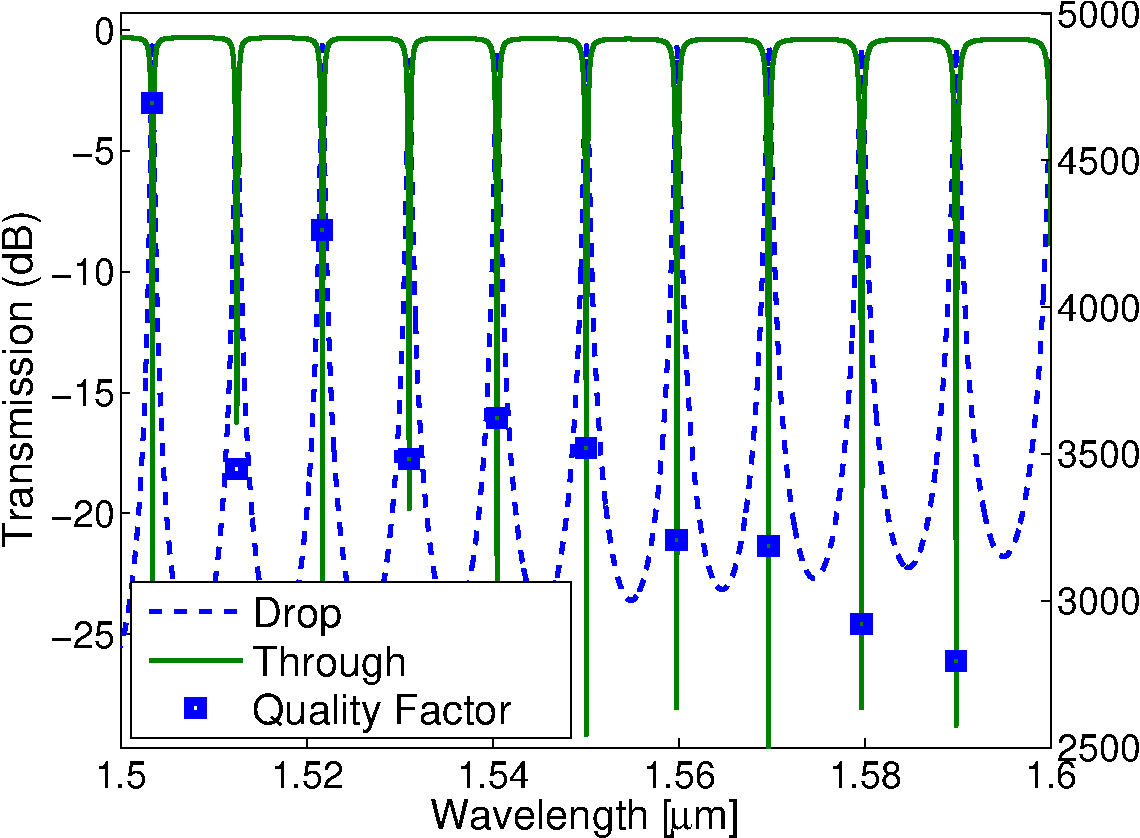
\includegraphics[width=0.4\linewidth]{../figs/a_1}
%\caption{Optical spectrum of the circuit in Figure~\ref{INT_DC}, in Lumerical INTERCONNECT.  The S-parameters shown in Figure~\ref{Fig-VF2a}-\ref{Fig-VF2p} are used for the directional coupler.  }
%\label{INT_ONA_DCring}
%\end{center}
%\end{figure}



\section{Schematic-Driven Layout}    

Prior to the advent of modern EDA tools, considerable time was spent drawing polygons in the physical layout.  In the Schematic-Driven Layout (SDL) approach, the components and connections are already defined in the schematic, and the task is to  place the components and route the connections using the already-defined connectivity (Place and Route).  

Next, a new layout is created using the schematic component connectivity.  In this mode, both the layout and schematic are visible simultaneously, and the schematic components are semi-automatically (``AutoInst'') instantiated in the layout.  The instantiation is typically done in groups (e.g., first all the modulators, then all the pads, then all the grating couplers).  The ``AutoInst'' function tries to preserve the relative positions and orientation of all cells in the schematic.  During the layout, alignment tools are used to ensure that waveguide ports line up horizontally and vertically, to minimize the number of S-bends and keep the waveguides straight.  The layout is shown in Figure~\ref{layout_wdm2tx_unrouted}.

It is at this stage in the layout that the placement of components is established, with consideration for testing (Design For Test, or DFT).  Especially critical is the location of the optical input/outputs, and their relative position with respect to the electrical ones.  

\begin{figure}[tbp]
\centering
 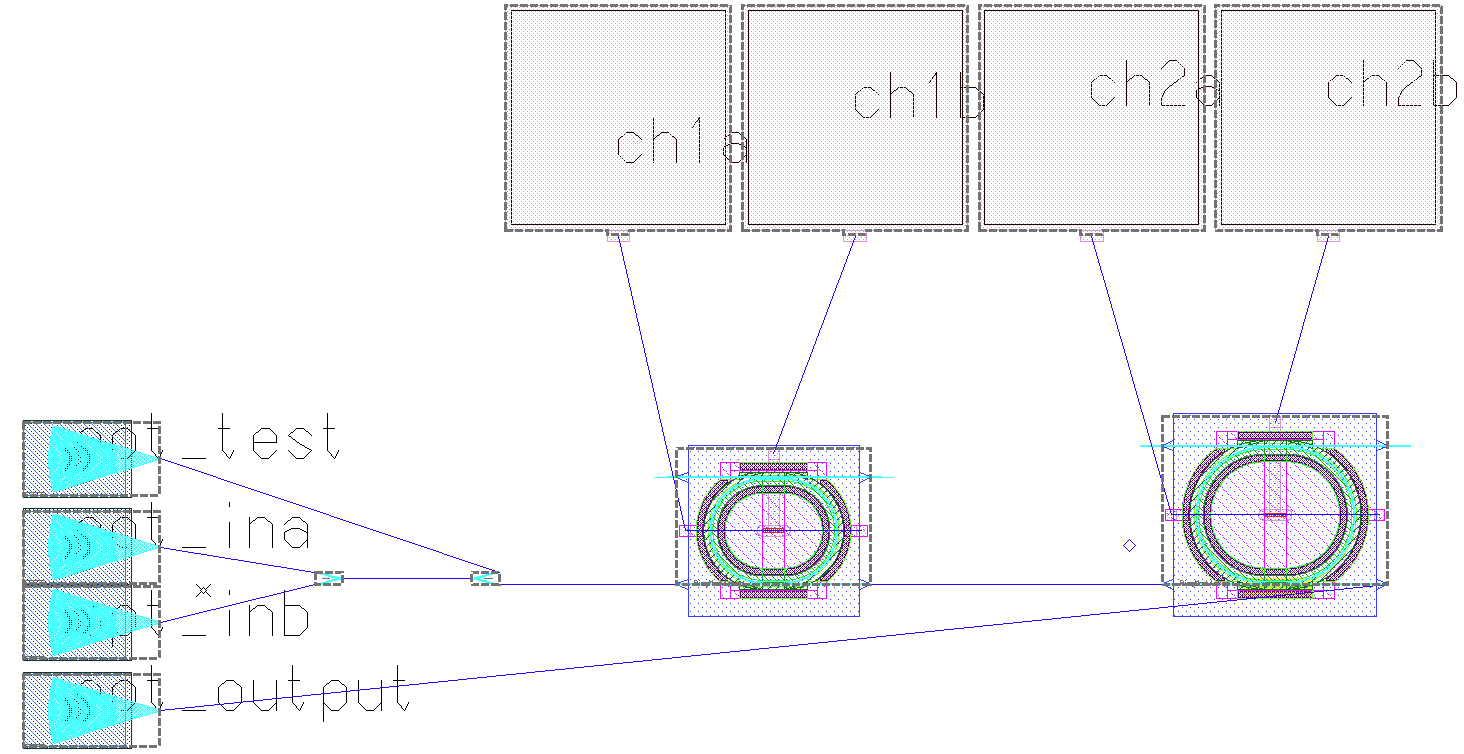
\includegraphics[width=0.7\linewidth]{../figs/layout_wdm2tx_unrouted} 
\caption{Layout for the example system, prior to routing.}
\label{layout_wdm2tx_unrouted}
\end{figure}

Next, electrical and optical routing is performed using the Pyxis ``IRoute'' interactive routing tool.  This creates path objects for both electrical and optical routes, and the optical routes have sharp 90$^\circ$ corners, as shown in Figure~\ref{layout_wdm2tx_routed}.

\begin{figure}[tbp]
\centering
 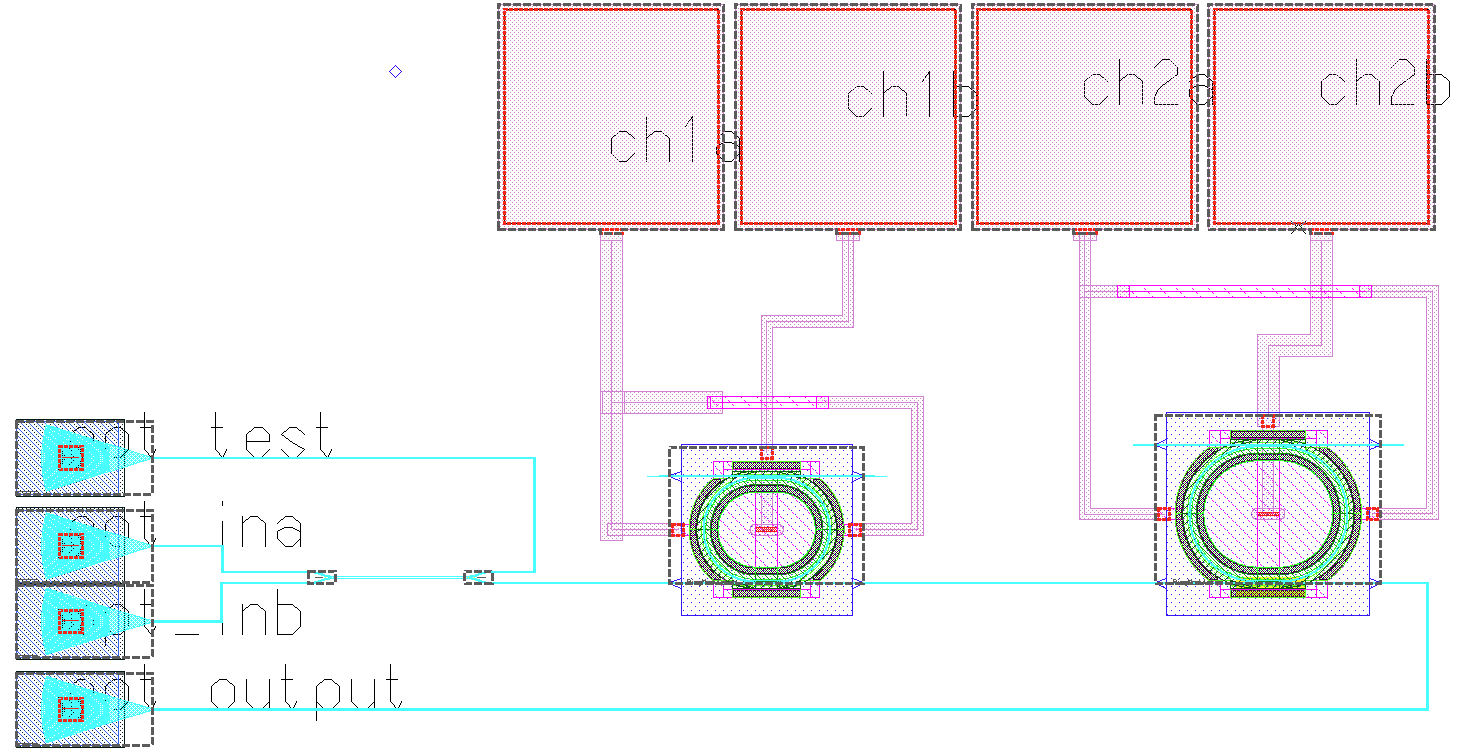
\includegraphics[width=0.7\linewidth]{../figs/layout_wdm2tx_routed}
\caption{Layout for the example system, after routing.}
\label{layout_wdm2tx_routed}
\end{figure}

The optical routes are then converted to optical waveguides.  This is done using the ``Make PWGs'' function.  This function implements the following features:
	\begin{itemize}
		\item Waveguide bends: instead of a 90$^\circ$ perpendicular corner like in metal interconnects (Figure~\ref{BezierBends1}), optical waveguides require smooth bends, which can be in the form on radial bends (Figure~\ref{BezierBends2}), or other adiabatic curves \cite{bogaerts2011compact, cherchi2013dramatic} (Figure~\ref{BezierBends3}).  The choice in the bend parameters is dependent on the performance requirements (insertion loss, back-reflections), the type of waveguide, the wavelength and the polarization (e.g., TM modes require larger bend radii).  This PDK gives the designer the choice of radius and bend type (radial versus adiabatic bezier), and is defined for different types of waveguides (strip, rib).

		\begin{figure}[tbp]		\centering   
		\subfloat[Corner for metal routing paths]{\label{BezierBends1} 
\includegraphics[width=0.2\linewidth,page=1,angle=180]{../figs/Bends1-key-crop.pdf} } ~ ~
		\subfloat[90$^\circ$ arc (radial bend)]{\label{BezierBends2} 
\includegraphics[width=0.2\linewidth,page=2,angle=180]{../figs/Bends1-key-crop.pdf} } ~ ~
		\subfloat[Adiabatic bend (Bezier curve)]{\label{BezierBends3} 
\includegraphics[width=0.2\linewidth,page=3,angle=180]{../figs/Bends1-key-crop.pdf} } 
		\caption{Possible 90$^\circ$ bends for metallic and optical interconnects.}
		\label{BezierBends}		\end{figure}	



The dominant loss mechanism in strip waveguides (for TE polarization) is mode-mismatch loss, which can be reduced by varying the curvature continuously.  An adiabatic $90^{\circ}$ bend based on a Bezier curve can have a lower optical insertion loss than a traditional arc with a constant radius of curvature.  This structure has been modelled for TE polarization at 1550 nm in strip waveguides.  The Bezier parameter describes the variation from a constant radius (Bezier=0.45) to a natural Bezier curve (Bezier=0). As shown in Figure~\ref{bezierresults}, much lower losses are achieved for the adiabatic bends based on Bezier curves.  The best $5 \mu m$ bend has the same performance as a radial $20 \mu m$ bend, whereas the best $3 \mu m$ bend has the same performance as a radial $6 \mu m$ bend.  Hence, these bends are more compact for the same allowable insertion loss.  The designer must choose the appropriate parameter based on the waveguide operation.  It should be noted that there is little improvement in using adiabatic bends for TM polarization since the dominant loss mechanism is radiative loss, as opposed to mode-mismatch loss.

		\begin{figure}[tbp]
\centering
		  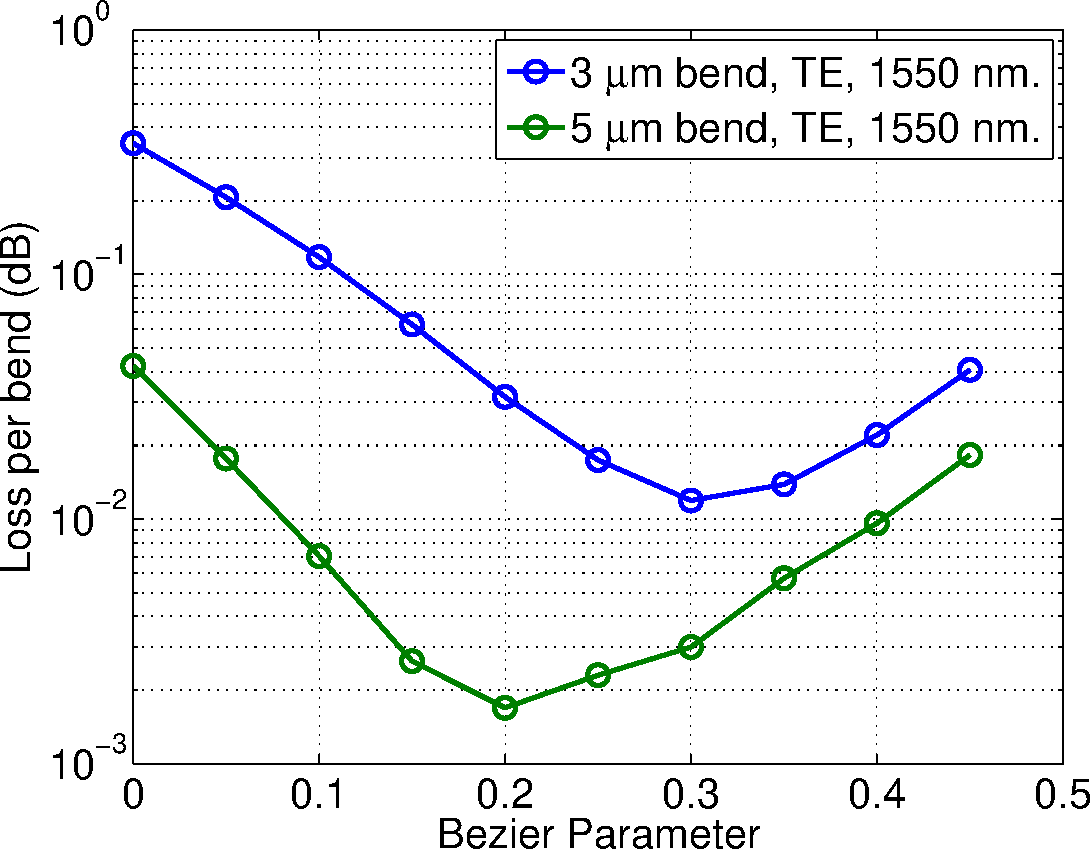
\includegraphics[width=0.5\linewidth]{../figs/bezier_bendloss1.pdf}
		    \caption{3D FDTD simulation results for the Bezier bends for $L=3 \mu m$, and $L=5 \mu m$.  Note that when the bezier parameter is 0.45, this is approximately a conventional arc with constant radius.  }
		\label{bezierresults}
		\end{figure}

		\item S-Bends: This structure is used to smoothly connect two disjointed and offset straight waveguides.  Optionally, it is automatically inserted when necessary.
		\item Automated augmented waveguides: for long distance optical routing, it is desirable to use lower-loss waveguides.  This is done by converting from a strip waveguide in the bend regions to a wide rib waveguide \cite{bogaerts2011compact, li2012ultralow-loss}.  The wide waveguides can be either single mode (700 nm wide with 0.27 dB/cm loss in Ref.~\cite{bogaerts2011compact}) or multi-mode (3 $\mu m$ wide with 0.026 dB/cm loss in a passive process, and 0.75 dB/cm loss in a full-flow, Ref.~\cite{li2012ultralow-loss}).  Experimental results for devices fabricated by IME in a full-flow process show that the propagation loss is $<$0.06 dB/cm for waveguides with a 3 $\mu m$ wide rib and a 5 $\mu m$ slab.  
		
		This PDK implements an optional automated waveguide augmentation.  The parameters include a length threshold for when to use the augmentation, a taper length, and the waveguide width.
		
		\item Waveguide crossings: Unlike electrons, photons can cross each other without interacting.  This simplifies the fabrication process since it does require multi-layer routing (as in electronics).  Low-loss and low-crosstalk waveguide crossings have been designed and fabricated \cite{bogaerts2007low-loss, zhang2013a-cmos-compatible}, and have been used in routing, and incorporated into devices such as ring resonators \cite{bogaerts2007low-loss}.  The crossings can be added by the designer similar to the other components.
	\end{itemize}


\begin{figure}[tbp]
\centering
 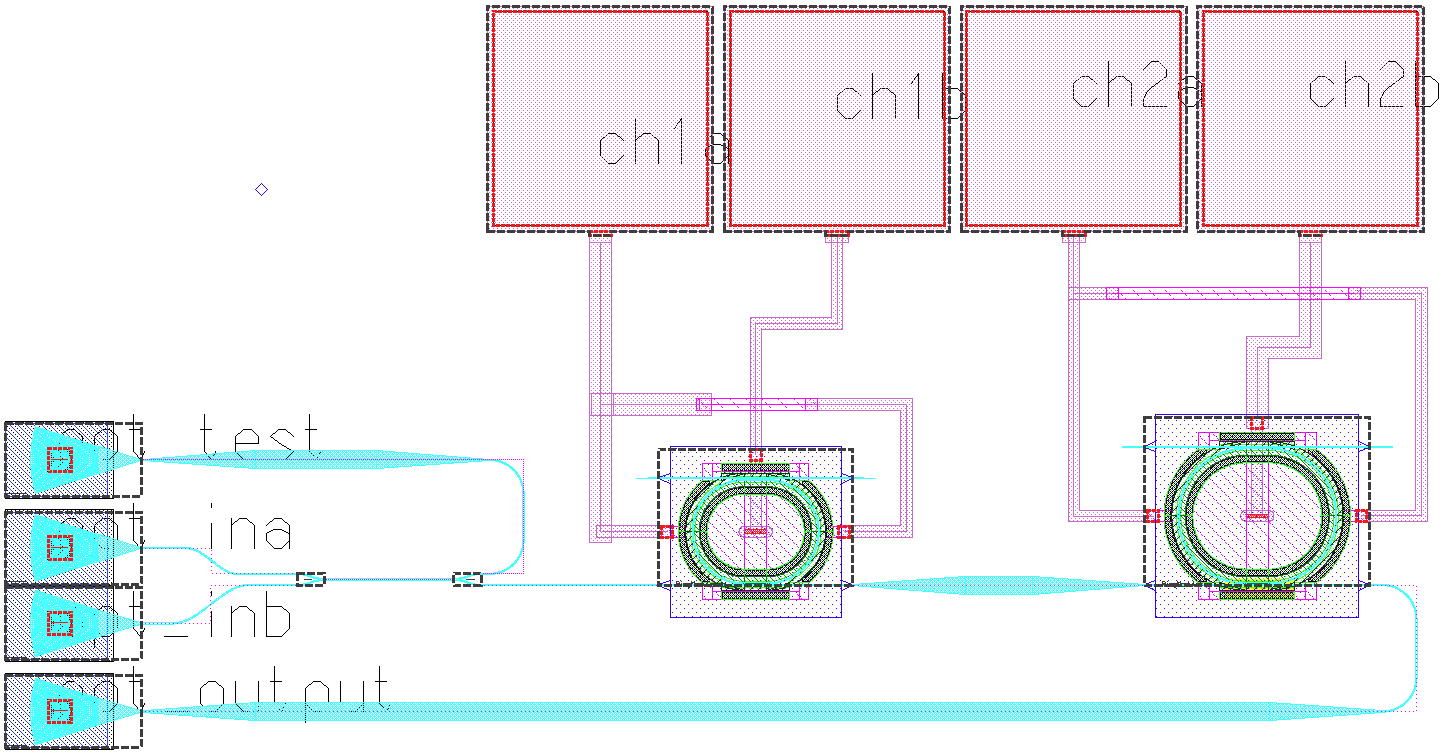
\includegraphics[width=0.7\linewidth]{../figs/layout_wdm2tx_done}
\caption{Layout for the example system, with optical paths converted into waveguides.}
\label{layout_wdm2tx_done}
\end{figure}

\section{Design Rule Checking}

%In this example, the minimum feature size and minimum spacing are defined for the silicon layer to be 200 nm.  A DRC rule file for a foundry may consist of 100s of rules.  

The rule checker operates in two modes: 1) Interactive -- as the layout is constructed, the tool graphically reports the errors; this allows the designer to correct the errors immediately during layout.  This is shown in Figure~\ref{DRC1}.   Interactive checking operates on a small fraction of the layout, namely the portion of the layout that is being edited and in view.  2) Sign-off verification -- the full layout is exported and checked for errors.  An error report is provided graphically and as a list.


\begin{figure}[tbp]
\centering   
\subfloat[Minimum space error flagged. ]{\label{DRC2a} 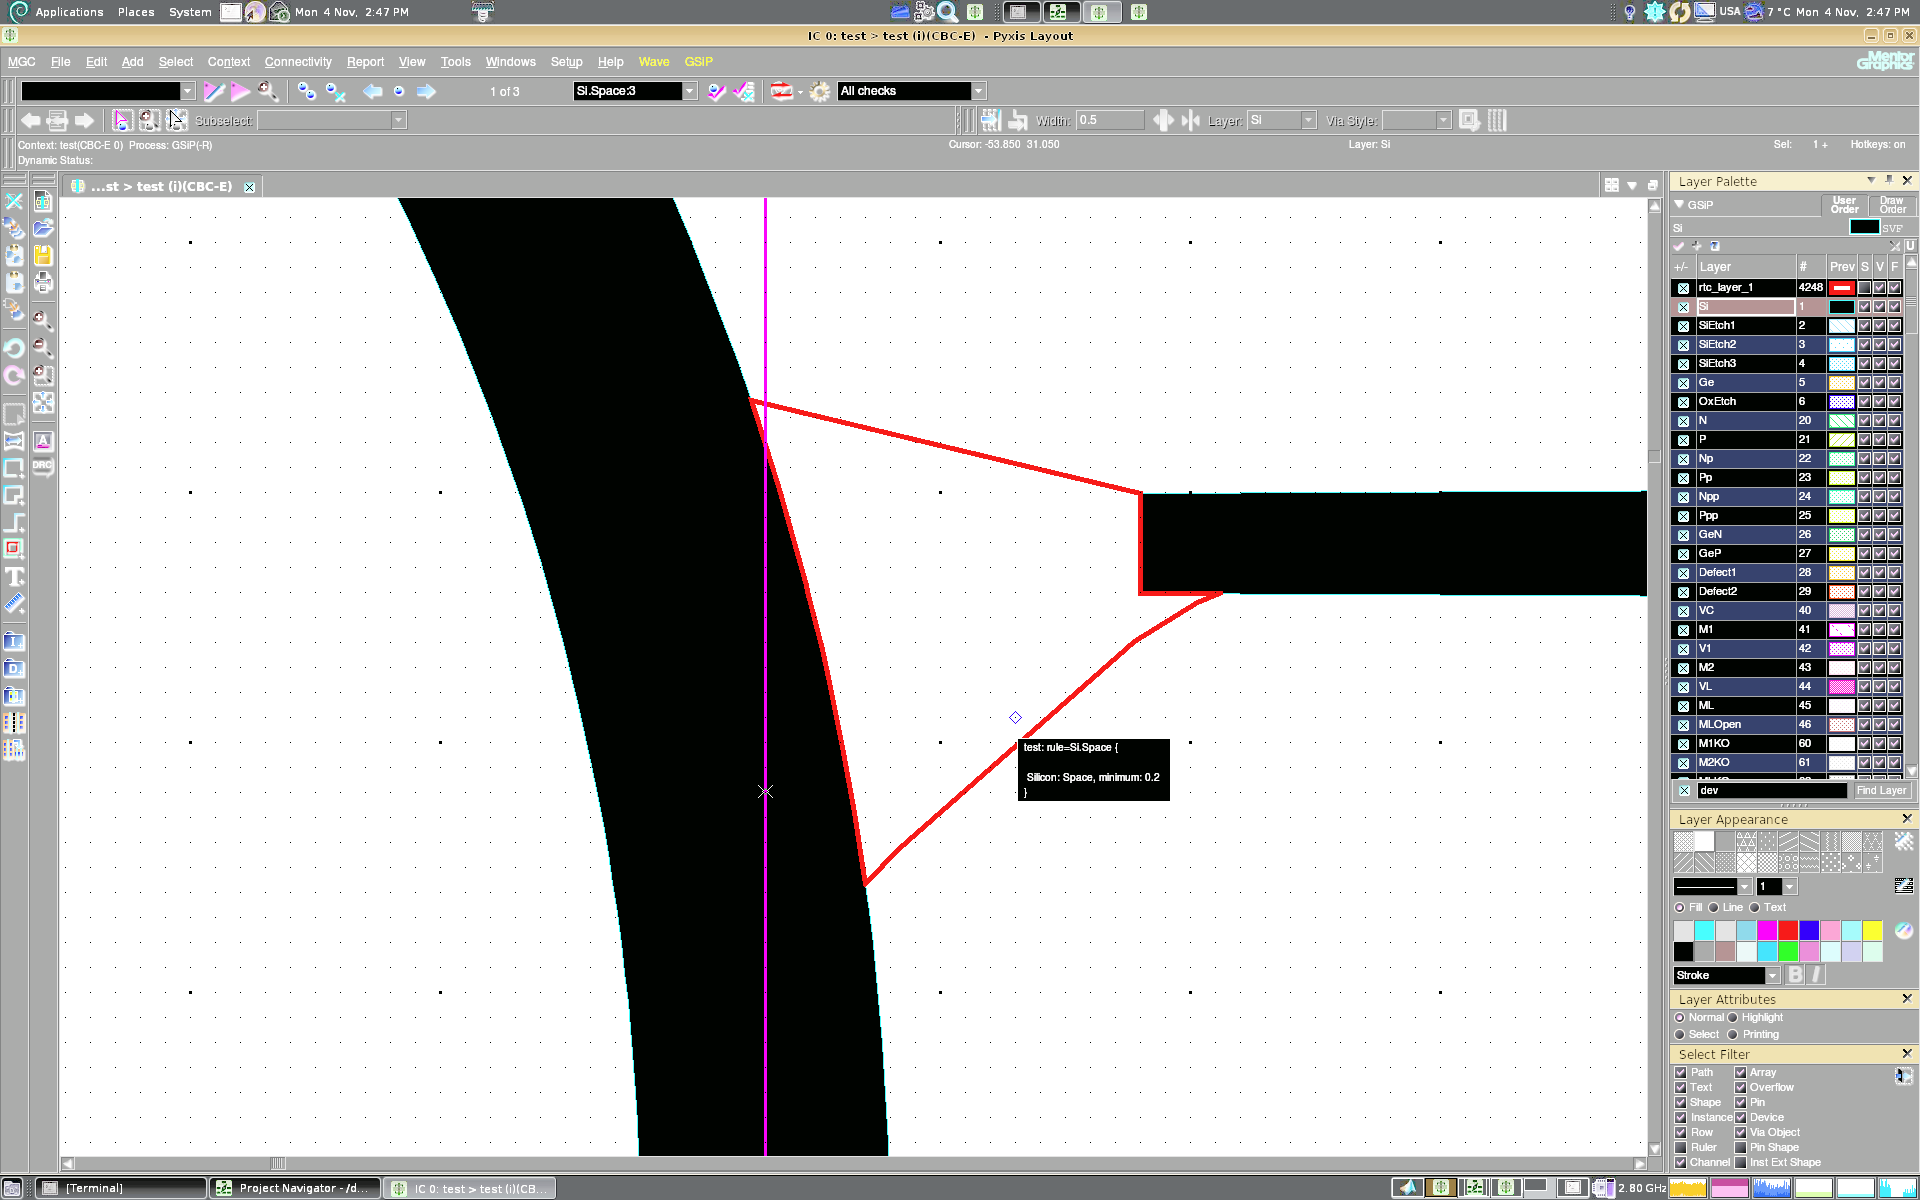
\includegraphics[width=0.47\linewidth]{../figs/DRC2a} }  ~ 
\subfloat[User fixes error; flag is removed. ]{\label{DRC2b} 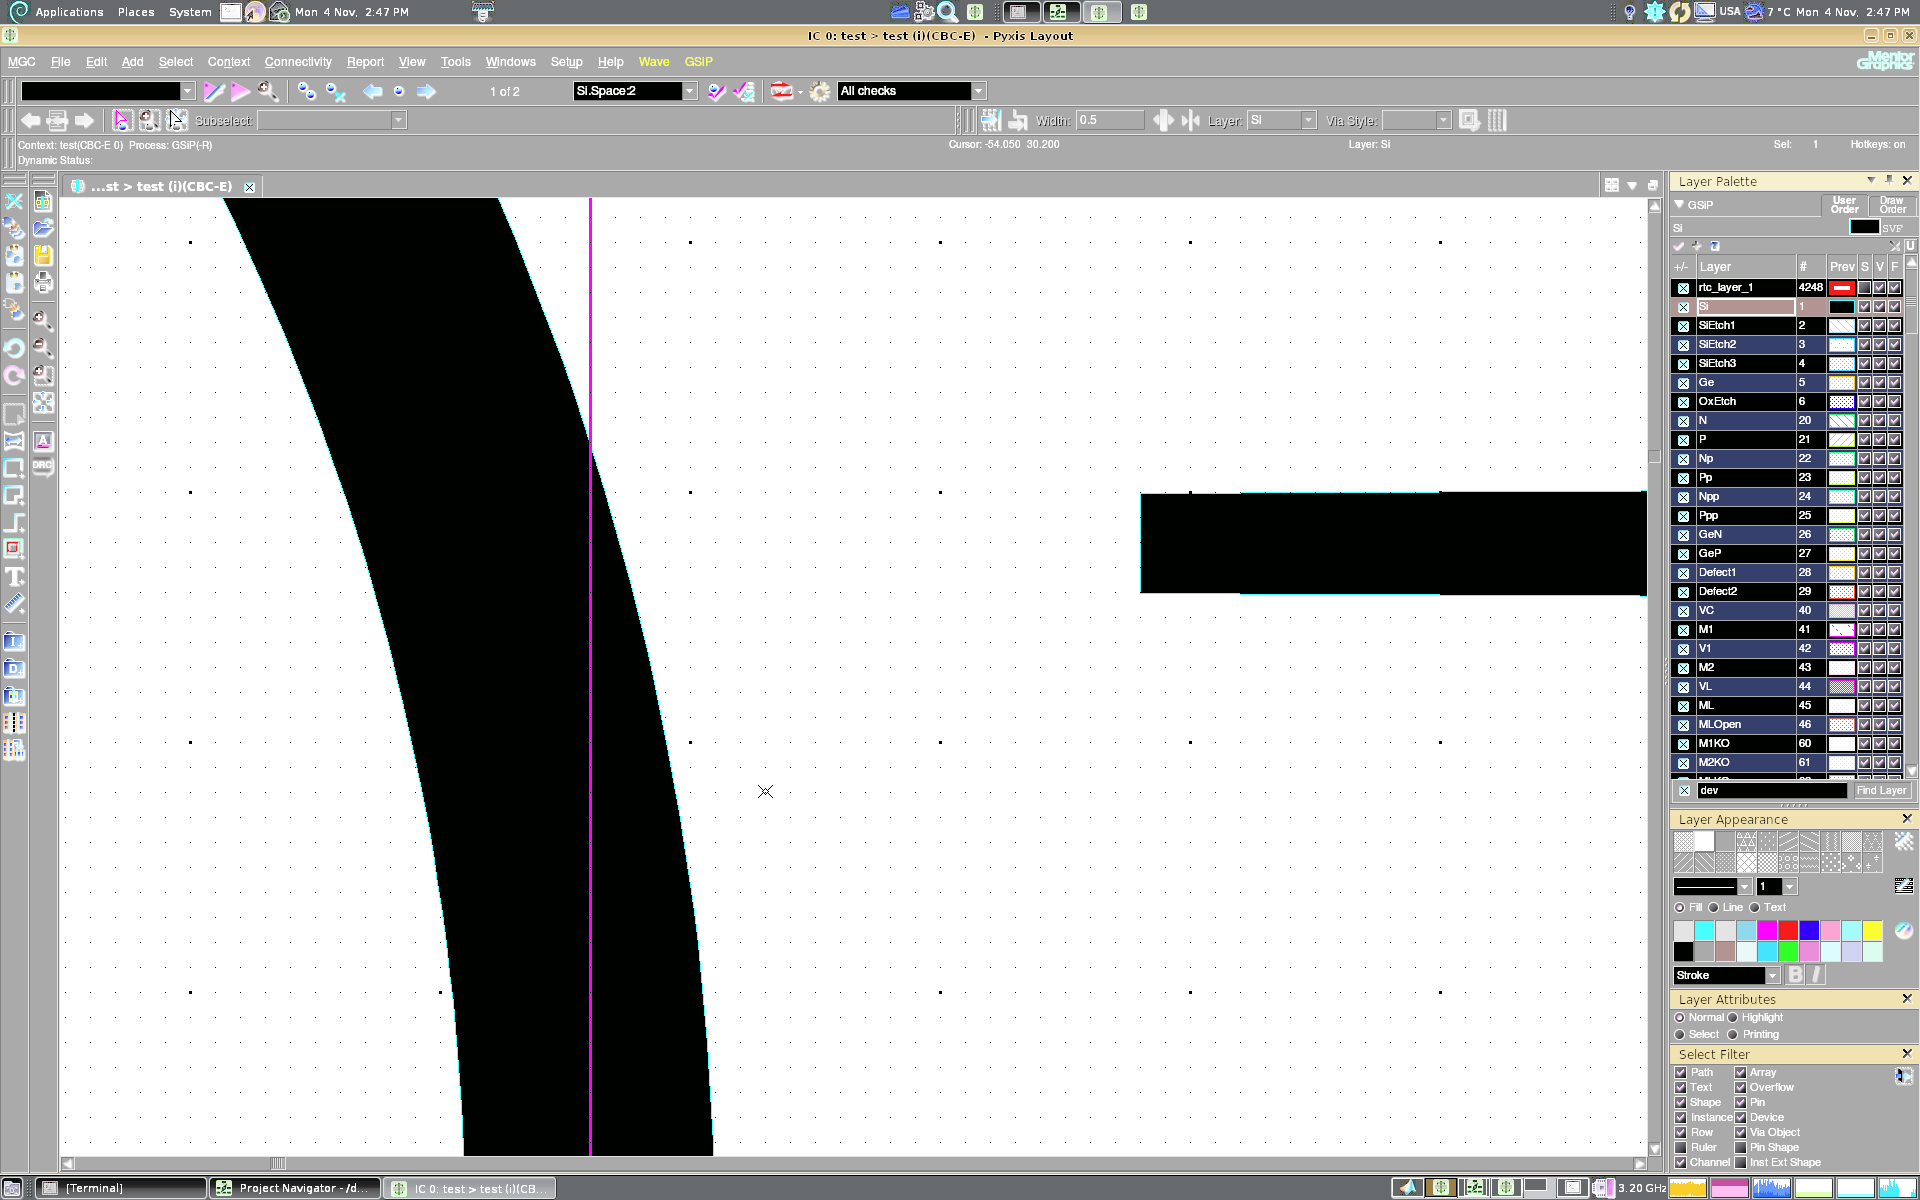
\includegraphics[width=0.47\linewidth]{../figs/DRC2b} }  
\caption{Interactive DRC checking, flagging errors while user is editing.}
\label{DRC1}
\end{figure}



\section{Layout Versus Schematic}

The first task in Layout Versus Schematic (LVS) is for the software to parse the mask layout file and identify structures from the drawn shapes.  The software  performs an extraction to finds known devices (e.g., ring modulator, grating coupler, etc.) and then determines their connectivity.  It  creates a netlist based on the layout, and compares it with the original schematic netlist.  

The extraction makes use of device recognition layers to simplify the process.  The first layer (``devrec'') is used to mark the extent of a particular device with a polygon, as well as to mark the area with a text label identifying the device name (e.g., ``RingModulator'').  The second layer (``pinrec'') is used to mark the location and name of the pins; both electrical (e.g., anode1, anode2, cathode), and optical (e.g., opt\_a2, opt\_b2).  A series of logical operations are used to find the geometries within the device recognition layers.  Measurements are then performed to extract the device parameters (e.g., gap in a directional coupler).  Additional operations are performed to find the connectivity between components.  


\section{Lithography, Fabrication Non-Uniformity}


One of the important issues with these silicon photonics fabrication is that small features, such as those found in Bragg gratings, are extremely sensitive to fabrication imperfections. For example, the corrugations in Bragg gratings are often designed to be square in the original mask layout. Unsurprisingly, however, the actual fabrication rounds the sharp corners, especially when using optical lithography \cite{wang2011uniform}. As a result, there is a significant performance mismatch between the originally designed (modelled) device and the actually fabricated device; specifically, the experimental bandwidth is usually much narrower than designed \cite{wang2011uniform}.    One solution to this problem is to include the fabrication process into the design flow \cite{bogaerts2008closed-loop}. Mentor Graphics provides an advanced lithography simulation tool to simulate the fabrication of devices fabricated with deep-ultraviolet (DUV) lithography \cite{adam2003improved}. After lithography simulation, the virtually fabricated devices can be re-simulated, to obtain a better prediction of the forthcoming experimental results \cite{wang2012lithography}.  

Future work in the design flow presented includes incorporating these lithography effects, thereby allowing the designer to simulate the circuit behaviour while taking into account lithography effects.  This will also allow designers to optimize their devices while taking into account lithography.

Photonic integrated circuits (PICs) often require precise matching of the central wavelength and the waveguide propagation constants between components on a chip (e.g., ring modulators, optical filters), particularly for wavelength division multiplexing.  Understanding the fabrication variability is critical to developing strategies (e.g., thermal tuning) for system implementation, and for determining the cost implications for such compensation strategies (e.g., power consumption). 
There have been several studies on the fabrication non-uniformity including intra-device uniformity (e.g., CROWs \cite{cooper2010235-ring}), within wafer, wafer-to-wafer, and batch-to-batch variations \cite{zortman2010silicon, krishnamoorthy2011exploiting, selvaraja2010subnanometer, wang2012narrow-band}.   The dominant fabrication parameter that results in device variation has been identified to be the silicon thickness variation, followed by lithography (e.g., waveguide width) variations.

Future work will address fabrication non-uniformity within the design flow.  This can be in the form of a process corners analysis (e.g., fast, slow), or preferably an analysis that takes into account the physical distance between devices in order to include distance correlation effects.  We have determined that the variation in multiple devices is strongly correlated to the distance between them \cite{chrostowski2014impact}.  Process corner analysis provides the variations observed on an absolute scale (i.e., wafer-to-wafer, batch-to-batch), but neglects on-chip correlation of process parameters which leads to reduced on-chip device variation.  The implication is the importance of very compact layouts when components need to be matched, leading to reduced (but not eliminated) trimming cost.  



\section{Conclusion}\label{sec6}

The opportunity for silicon photonics is to leverage three decades of CMOS Electronic Design Automation (EDA) tool development, and two decades of optical design software development.
Full-flow design environments are becoming a reality for silicon photonics.

The mature CMOS fabrication processes and multi-project wafer (MPW) fabrication runs 
%Stable processes that are repeatable
enable the development of component libraries for system design.  Emphasis needs to be placed on developing parameterized components to bring increased utility for system-level design, and incorporating manufacturing yield and process variations into the design flow.  

Similar to the electronics industry, photonic integrated circuit design and fabrication is evolving towards specialized roles, namely: a) fabrication and processing, b) EDA tools; c) component, library, and PDKs; and, d) system design.  This separation of roles will lead to accelerated product development and ultimately aiding the silicon photonics industry achieve its objectives. 



\acknowledgments

The authors would like to thank CMC Microsystems for enabling the fabrication of numerous chips via imec-ePIXfab and IME. 
Funding for this research was provided by NSERC, particularly the NSERC CREATE Silicon Electronic Photonic Integrated Circuits (SiEPIC) training program, \url{http://www.siepic.ubc.ca}.
The authors are grateful to Nicolas A.F.~Jaeger and Tom Baehr-Jones for useful discussions. 

\bibliography{../Refs/references}
\bibliographystyle{spiebib33}


\end{document}
